% !TEX encoding = UTF-8
% !TEX TS-program = pdflatex
% !TEX root = ../nt.tex
% !TEX spellcheck = it-IT

%************************************************
\chapter{Modeling}
\label{cap:mdlng}
%************************************************\\

\section{Progettazione}

Dal punto di vista ingegneristico i costi di progettazione di una Ferrari e di una Fiat non sono poi così differenti. La reale differenza risiede nel modo in cui i due differenti progetti sono ottimizzati per lo specifico target di clientela e per le caratteristiche ed aspettative, evidentemente differenti, delle due automobili. Un ingegnere progetta qualcosa di \textit{customizzato}, cioè creato su misura per il committente, di fatto proiettando un’idea che risiede nella sua mente. A differenza di un progettista di automobili o di edifici, un progettista del software è in grado di interagire con la mente delle persone e di cambiarne le idee. 

\subsection{Caso di Studio - Google}

Oggigiorno i Database sono ovunque. Google è uno dei DB più diffusi. Quando viene effettuata una ricerca in realtà viene eseguita una query per comunicare con il SW di Google. La successiva figura illustra un sistema \textbf{\textit{Client/Server}} per interrogare un Database. Un \textbf{DBMS} (\textit{Database Management System}) è un sistema che consente di gestire uno o più DB.

\begin{center}
\begin{figure}[H]
\centering
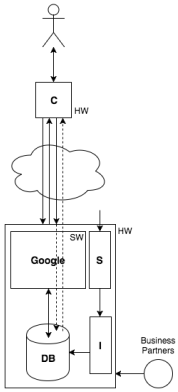
\includegraphics[scale=1]{figures/cs.png}
\caption{Architettura Client-Server} 
\end{figure}
\end{center}

La nuvola rappresenta Internet, un insieme dinamico di connessioni, mentre il Client è una macchina (HW) al cui interno risiede il SW. Tramite l’inserimento dell’url nel browser viene generato un round-trip. Una volta stabilita la connessione con il DBMS sarà possibile accedere alle informazioni che risiedono nel DB. Ad esempio la ricerca delle parole: “Cinema Lecce” restituirà tutte le occorrenze dell’intersezione degli insiemi costituiti dai risultati di ricerca delle due singole parole. Sui computer di proprietà di Google oltre al DBMS esistono altri software: \textbf{Spider} o \textbf{Crawler} e \textbf{Indexer}. 

Supponiamo che il web sia un grafo connesso, ovvero che ogni pagina web che risponde ad un url contenga i riferimenti (url) ad altre pagine web e così via, fornendo un url allo Spider esso ricorsivamente percorre tutto il grafo passando ciascuna pagina visitata all’Indexer. L’Indexer ha il compito di effettuare lo stamming delle parole ovvero la loro estrazione ed il mantenimento dei riferimenti alle pagine cui sono state trovate. L’idea pertanto consiste nel mantenere un indice analitico delle parole e i riferimenti a tutte le pagine web che le contengono. Questo consente di riuscire ad immagazzinare tantissimi riferimenti utilizzando pochi gigabytes. Quindi quando vogliamo effettuare una ricerca nel web ricorrendo ad un motore di ricerca le ricerche in realtà sono state già effettuate e l’unica cosa che fa il software è incrociare le informazioni. Google viene pagata da altre grosse società per far salire in cima i risultati delle ricerche per i contenuti che le riguardano. Osserviamo che l’ipotesi di rappresentazione del web attraverso un grafo connesso non è rappresentativa di alcune realtà come quella del deep web. Il deep web è costituito da isole cioè porzioni di grafo non connesse a quelle del web pertanto non raggiungibili sebbene nelle isole vengano utilizzati gli stessi protocolli del web (HTTP, ecc.).   

\subsection{Organizzazioni}

Per quanto concerne le persone che hanno a che fare con un sistema SW, possiamo distinguere tre tipologie principali: \{\textbf{User}, \textbf{Consumer}, \textbf{ Customer}\}. Per quanto riguarda le modalità di interazione e comunicazione con un sistema SW, troviamo la tipica architettura \textbf{\textit{Client-Server (C/S)}} e la \textbf{\textit{Peer-to-peer (P2P)}}. Nel P2P le entità in gioco sono tutte alla pari, nel senso che avvengono degli scambi alla pari di informazioni. Internet è oggigiorno dominata da questi due meccanismi. Abbiamo cominciato a vedere una prima tipologia, gli user, che sono però una parte di tutto il resto: gli \textbf{stakeholders} che letteralmente sono dei portatori di interesse, qualcuno interessato ad un sistema. Gli \textbf{UT} (\textit{User Types}) sono un sottoinsieme degli Stakeholders. Ad esempio, il rettore è uno stakeholder, ma non un utente. A volte sono proprio loro che comandano il tutto! Egli potrebbe pure non interagire con il SW, decide però le regole in gioco. Per parlare di uno stakeholder bisogna necessariamente precisare il sistema: per Google ad esempio, Ferrari è uno stakeholder particolare, denominato \textbf{business partner}. 
Parliamo ora di \textbf{Sistema} ed \textbf{Organizzazione}. Cos'è un'organizzazione? Esistono le persone e poi le organizzazioni. L'Università è un tipico esempio di organizzazione: struttura di persone che svolgono dei compiti ed hanno delle responsabilità, esse si occupano tipicamente di prodotti e di servizi. All'interno di un'azienda non vi può essere soltanto il singolo venditore, tipicamente vi è anche una fitta rete di assistenza. Noi abbiamo sempre a che fare con bundle di prodotti e servizi, ad esempio il comune telefono è un prodotto ed un servizio allo stesso tempo pertanto oggi quasi tutto è quindi un bundle di prodotti e servizi.  
Per schematizzare una tipica organizzazione possiamo avvalerci del modello di Anthony, che prevede una suddivisione piramidale dell'organizzazione in tre parti o livelli: Direzione, Management ed Operativa. Nell'Università ad esempio abbiamo il rettore, i presidi ed i professori e tecnici, stesso discorso per banche, ospedali, etc. La direzione è costituita da uno o pochi individui o da un consiglio di amministrazione, poi c'è il manager, il quale non è il capo dell'azienda: è il vice-capo ma risponde al direttore. I manager sono, nell’esempio dell’università, i direttori di dipartimento. Il personale operativo è chiamato anche \textbf{Front Office}. Svolgere i compiti operativi all'interno dell'università. Non bisogna però confondere Ruolo e Persona. L'organizzazione può essere rappresentata da un \textbf{organigramma}, la carta che rappresenta gli organi che compongono l'azienda e che rappresentano, tipicamente, una struttura gerarchica. Le organizzazioni, per essere ben guidate, a meno che non presentino strutture di tipo rete, devono essere strutturate in modo gerarchico, in alcuni casi vi potrebbe addirittura essere una replicazione del modello gerarchico. Nel caso delle holding ad esempio la struttura è di tipo gerarchico ed ogni organizzazione costituente è a sua volta una struttura gerarchica. Il \underline{sistema informativo} esiste da sempre e non è costituito da bit! Esso è costituito da informazioni. Il \underline{sistema informatico} è rappresentato da computer e dalle reti. 
 
Sebbene le informazioni esistano da sempre il sistema informatico è piuttosto recente, infatti nel tempo può cambiare il processo di elaborazione delle informazioni, il quale insieme alle informazioni stesse costituisce il sistema informativo. Attualmente il sistema informativo esiste su sistemi informatici ma prima dell’avvento dei computer “viveva” sulla carta.  
Come si crea un sistema informativo per un particolare ruolo? Ad esempio, per un direttore, preside o professore. Il ruolo è svincolato dal soggetto fisico! Lo stesso Anthony, con la sua piramide, ci fornisce un grande supporto per l'attività di Analisi dei Requisiti. Sempre riferendoci alla struttura piramidale, possiamo individuare altri tre livelli che meglio identificano e raggruppano i differenti tipi di dati che vengono trattati dai ruoli che appartengono ai tre differenti livelli gerarchici: La \textbf {BI} (\textit{Business Intelligence}), l'\textbf{ERP} (\textit{Enterprise Resource Planning}), ed il \textbf{CRM} (\textit{Customer Relationship Management}). Nel primo livello troviamo tipicamente sistemi DSS (\textit{Decision Support Systems}). Invece nello strato intermedio troviamo sistemi per la gestione e pianificazione delle risorse all'interno di un'azienda. SAP ad esempio, nato inizialmente in seno ad IBM, produce software ERP per le aziende.  
Le risorse di un sistema si suddividono in: \textbf{RI} (\textit{risorse immateriali}), \textbf{RM} (\textit{risorse materiali}) e \textbf{RU} o \textbf{HR} (\textit{risorse umane, human resources}). L'Università, gestisce solo le informazioni dello studente! Le RM sono tangibili. Le RU sono il professore, i tecnici, gli amministrativi. Questi software, o sistemi più in generale, sono molto importanti e complessi allo stesso tempo. L’acronimo CRM sta per Customer Relationship Management, a questo livello sono immagazzinati i dati degli acquisti dei clienti e si possono attuare delle tecniche MBA, ovvero di Market Basket Analysis. Nei vari sistemi superiori al CRM, per aggregare i dati in informazioni di livello superiore, si sfruttano delle potenti tecniche di clustering, Business Intelligence e Machine Learning. Con questi sistemi possiamo digerire quantità potenzialmente grandi di dati. Le informazioni possono essere di tipo analitico e di tipo sintetico. A livello CRM abbiamo ad esempio solo informazioni analitiche, più dettagliate. Tali informazioni vengono via via aggregate nei livelli superiori, mediante tecniche di cui sopra. Ci siamo serviti quindi del triangolo DMO di Anthony per capire come funzionano le organizzazioni, le persone ed i processi che elaborano le informazioni. 
 
Un \textbf{database} è una raccolta di informazioni, il cui ciclo di vita può essere sintetizzato nell’acronimo \textbf{CRUD} (\textit{Create, Read, Update, Delete}). Le informazioni sono straordinariamente importanti. Sapere delle informazioni ci consente di procedere operativamente in determinate direzioni piuttosto che in altre. Imparare a progettare i sistemi informativi serve a risolvere concretamente vari problemi delle persone. Abbiamo quindi a che fare con un mondo di informazioni ed organizzazioni, le quali giacciono in complesse reti. Servono tecniche di modellazione e di soluzione del problema complessivo.  
Un'impresa consiste in delle risorse: RI, RM, RH. Qual è il valore associato a questi oggetti? Le risorse umane, dal punto di vista dell'organizzazione, hanno un enorme valore; costituiscono il valore stesso dell'azienda, sono delle risorse non alienabili la cui sostituzione può avere effetti negativi sull’azienda stessa. Anche le RM sono delle risorse importanti, possono essere vendute per creare valore. Tuttavia, rivestono una grande importanza le risorse immateriali, ovvero le informazioni. Basti pensare a cosa accadrebbe se venissero cancellati tutti i dati dal database dell'università!!! Le informazioni all'interno delle organizzazioni hanno un valore direttamente rapportabile a quello che l'organizzazione fa. Oggi il mercato è strutturato in: Primario, Secondario, Terziario e Terziario Avanzato. Noi ingegneri informatici ci collochiamo nel settore terziario. Facendo dei conti, considerando ad esempio il mercato telefonico, esso vale circa, a livello mondiale, un migliaio di miliardi di dollari. Questi soldi fanno girare un mercato enorme, ed in gioco vi sono degli interessi pazzeschi! Grandi aziende come Apple, Samsung, o Microsoft decidono del guadagno e della perdita di queste enorme moli di denaro. Oggi quando parliamo di Google o di Facebook, parliamo di tutto il mondo che c'è dietro. Trattano il settore della Comunicazione, ma lo mutano profondamente: "\textit{Bisogna creare il bisogno}", dicono gli esperti di marketing e dinanzi a una apparente frase banale, si celano queste importanti dinamiche, che un progettista informatico deve assolutamente sapere. Non si tratta più di questioni legate all'ottimizzazione del codice ad esempio! Le informazioni sono quindi le risorse fondamentali delle organizzazioni: è una dimensione molto importante da conoscere.  
 
Vediamo ora l'organizzazione come un Sistema Dinamico, che viene attraversato da input e produce in uscita degli output. Il direttore ha bisogno di conoscere i cosiddetti \textbf{KPI} dell'organizzazione (\textit{Key Performance Indicator}), per sapere se l'azienda sta andando bene o meno. Queste informazioni vengono interpretate attraverso il cosiddetto \textbf{cruscotto aziendale}. Alla stregua di una macchina, le aziende si guidano e chi le guida ha necessariamente bisogno di questo cruscotto. Le informazioni devono quindi essere sempre presenti. Un’organizzazione può essere vista come una black box, che riceve in ingresso Materie Prime ed informazioni, queste vengono elaborate mediante rispettivamente sistemi operativi ed informatici, e produce alla fine in output dei prodotti o servizi, ed altre informazioni. Troviamo i cosiddetti \textbf{EIS} (\textit{Enterprise Information System}) a tal proposito. 


\subsection{Lo scenario della progettazione - Progetto e realizzazione}

Come si colloca il concetto di modello nell’ambito dell’ingegneria? Consideriamo l’esempio dello scaldabagno: quando accendiamo il termostato la temperatura aumenta nel tempo con un andamento esponenziale fino a quando ad un certo punto non inizia a decrescere e così via. Una rappresentazione analitica di questo problema ci porterebbe intuitivamente a considerare la temperatura come una variabile rilevante mentre il colore della spia del termostato come una variabile irrilevante. Un \underline{\textbf{modello di analisi}}, quindi, è una rappresentazione minimale di un sistema fisico depurato dagli effetti secondari in cui possiamo identificare una relazione I/O utile ai nostri scopi. I \underline{\textbf{modelli di sintesi}} sono la concettualizzazione di un oggetto che sto creando.  Il \textbf{requisito} è il modo in cui si traduce la fattibilità tecnica del sistema che si sta progettando, i requisiti costituiscono le possibili soluzioni del problema. I Goal sono i motivi per cui mi rivolgo al progettista, essi vengono risolti dai requisiti. Il progettista ha l’obbligo di rendere al cliente dopo qualche giorno dall’intervista un modello concettuale (MC), un’astrazione del \textbf{modello fisico} del problema. Il \textbf{modello concettuale} deve rendere l’idea di come il progettista ha pensato di risolvere il problema, il tutto ricorrendo ad un linguaggio comprensibile per il committente e facendo uso di illustrazioni grafiche, i Mockups. Il progettista ha a disposizione pochissimi minuti per illustrare la sua idea al committente e a convincerlo della buona riuscita del suo lavoro. 
 
Dal momento che il committente in generale può essere incerto sulle richieste e potrebbe cambiarle in corso d’opera si redige un documento formale in cui si fissano i requisiti e si fanno firmare dal committente. Questa fase non è remunerativa pertanto è consigliabile non sprecare risorse economiche. Qualora il modello concettuale dovesse andar bene si firma un contratto tra le parti ed il committente è tenuto a dare un acconto. Il \textbf{modello logico} (ML) è un documento tecnico interpretabile da professionisti e tecnici esperti del dominio in cui sono contenute informazioni dettagliate circa lo sviluppo del progetto. Occorre definire uno standard di interfaccia tra il team e il progettista. Il team prende visione anche del modello concettuale ed infine produce il \textbf{modello fisico} (MF). Nella fase di progettazione iniziale è fondamentale predisporre anche tutti i casi di test nonché le possibili eccezioni per poi verificarle man mano che blocchi del software vengono costruiti. Il consulente è un professionista, generalmente un analista, che viene pagato dal committente per supervisionare esternamente tutto il processo di sviluppo del software e per curare i suoi interessi. Il suo compito consiste nel controllo del progettista, del team, supervisiona le release intermedie del SW e si occupa anche di collaudarlo. 

\begin{center}
\begin{figure}[H]
\centering
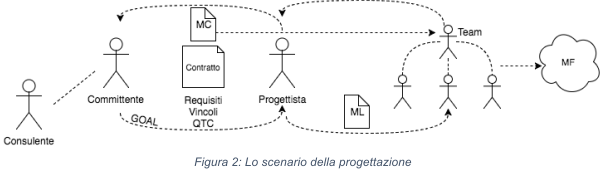
\includegraphics[scale=0.8]{figures/mdlng.png}
\caption{Scenario della Progettazione} 
\end{figure}
\end{center}

\begin{flushright}Marco Chiarelli\\Gabriele Accarino\\28/09/2016\end{flushright}

\subsection{Scenario Ingegneristico della Progettazione}

Goal + requisiti + vincoli + test = contratto

\begin{center}
\begin{figure}[H]
\centering
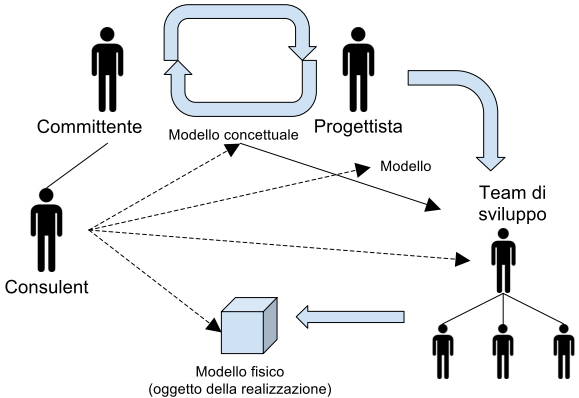
\includegraphics[scale=1]{figures/mdlng2.png}
\caption{Scenario della Progettazione} 
\end{figure}
\end{center}

Lo scenario tipico del progetto ingegneristico è il seguente: abbiamo un \textbf{committente} che richiede un \textbf{prodotto} (nel caso dell’ingegneria informatica, un’applicazione), un \textbf{progettista} che, parlando col cliente, estrae i goal del progetto, i requisiti, i vincoli di qualità, tempo e costo e i test da effettuare e dà al committente un documento, chiamato \textbf{modello concettuale} che conterrà le stime dei costi e del risultato finale del prodotto (nel caso di progetti legati al mondo dell’informatica, spesso corrispondono ai mockup) che si assocerà, alla fine, al \textbf{contratto}. Il progettista raffina il suo modello concettuale creando un altro documento che si chiama \textbf{modello logico} (che contiene i calcoli e specifiche tecniche maggiori di quelle presenti nel modello concettuale) e, insieme al modello concettuale, sarà la base da cui partiranno i \textbf{membri del team di sviluppo} (composta generalmente da un team leader e dagli sviluppatori) e si occupa di trasformare i modelli logico e concettuale, nell’\textbf{oggetto della realizzazione} (nell’ingegneria informatica corrisponde col \textbf{modello fisico}). Il committente, per assicurarsi che il lavoro sia corretto e con un buon rapporto qualità prezzo, si affida ad una terza figura, il \textbf{consulente} che, grazie alla sua esperienza pregressa, affianca il committente per verificare ogni fase del progetto.   
Le risorse materiali costano poco nella fase di sviluppo di un progetto dell’ingegneria informatica, il costo maggiore in un progetto lo si ha nelle risorse umane e immateriali. Avendo questa importante informazione, questo modello ci permette di fare una stima dei costi molto precisa: si utilizzano i \textbf{\textit{function points}} che, data una serie di specifiche, permettono di capire quanto tempo ci vuole per realizzarle. Dato il tempo di sviluppo in anni uomo, si può semplicemente moltiplicare questo valore per il costo annuo di uno sviluppatore per avere il costo totale del progetto. A questa documentazione bisogna aggiungere anche la \textbf{matrice RACI} che serve per dire “chi ha fatto una determinata parte del progetto” in modo da dare all’azienda produttrice la possibilità di tracciare la qualità di un ingegnere o di uno sviluppatore. Ricapitolando, un modello può essere fatto per il committente o per i membri del team ma, indipendentemente, è un insieme di regole e simboli noti (per esempio, in un modello dell’architettura di una casa, un segmento con un arco di circonferenza di 90 gradi indica una porta). Nel mondo dell’ingegneria informatica, i modelli statici e dinamici sono tipicamente logici, ma possono anche essere usati nel modello concettuale da mostrare al committente. Per esempio, se volessimo creare un gioco di scacchi, dovremmo creare nel diagramma delle classi una classe “casella”, una classe “scacchiera” (aggregazione di caselle), dopodiché si crea una classe generica “pezzo” che verrà implementata diversamente per ogni pezzo (pedoni, cavalli, alfieri, ecc…). Questo tipo di progettazione, dove il modello guida la progettazione, si chiama \textit{\textbf{model driven engineering}}. Si usano le tecniche di modellazione come quelle di \textit{\textbf{forward e reverse engineering}}. La prima permette, guardando il modello, di creare il software; viceversa la seconda. Ogni tipo di progettazione ha un limite. Nel caso della progettazione \textit{model driven} si ha che il \textit{reverse engineering} ha un costo e non è del tutto automatico, quindi ciò porta ad avere casi in cui si inizia creando il modello, si crea il codice e si modifica la struttura senza modificare il modello. Se si cambiano parti di un progetto senza modificare il modello a lungo andare si dimenticherà il motivo di tale modifica. Per questo motivo sono nati i processi di \textbf{BPR} (\textit{business process re-engineering}). Tale processo, chiamato anche “prato verde”, permette ai nuovi team di evolversi autonomamente, senza l’obbligo di seguire metodi precedentemente utilizzati.


\section{Architettura di un Progetto Software}

\subsection{L'hardware}

Ogni calcolatore è basato sul modello della macchina di Von Neumann che presenta una parte logica (CPU), una o più memorie, uno o più dispositivi di input/output e un bus che collega il tutto. 

\begin{center}
\begin{figure}[H]
\centering
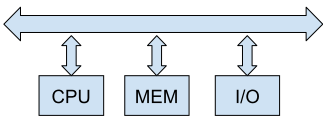
\includegraphics[scale=1]{figures/vonmn.png}
\caption{Modello della macchina di von Neumann} 
\end{figure}
\end{center}

La CPU contiene le unità ALU (\textit{Arithmetic and Logic Unit}), FPU (\textit{Floating-Point Unit}), CU (\textit{Control Unit}) e dei registri. La memoria contiene i programmi (la sequenza di istruzioni) e i dati. In questo modello, il calcolatore, al suo avvio, esegue l’istruzione alla posizione numero 0, poi la sua successiva e così via in \textbf{sequenza}. Il modello di Von Neumann permette anche di variare il flusso di esecuzione, attraverso la comparazione e il salto. Possiamo dividere un’architettura software in diversi livelli. Il primo livello che si può trovare è il \textbf{livello hardware}, che si basa sul modello della macchina di Von Neumann. Il livello successivo è il \textbf{livello macchina} che implementa le istruzioni di esecuzione (DO), di comparazione (CMP) e di salto (JMP) nel linguaggio macchina. Questo tipo di programmazione è di tipo \textbf{imperativo sequenziale}. La sequenza può essere variata tramite CMP e JMP. Il linguaggio macchina è composto da un alfabeto di 2 caratteri (0 e 1) quindi troppo di basso livello per l’essere umano. I linguaggi che implementano queste istruzioni si chiamano \textbf{linguaggi assemblativi} (Assembly è il più famoso), nel corrispettivo livello (\textbf{livello assemblativo}). Un comando a livello assemblativo corrisponde a una serie di istruzioni a livello macchina. Il risultato di questo tipo di programmazione è anche chiamato \textbf{codice spaghetti}, dato dal grande numero di salti tra le varie righe di codice. Il \textbf{linguaggio strutturato} viene introdotto per ridurre gli errori causati dal livello assemblativo, ancora di livello troppo basso e per l’eccessiva libertà che si ha nel programmare. I linguaggi che fanno parte di questa categoria sono il C, il FORTRAN, il Pascal, e il Basic. La caratteristica di questi linguaggi è quella di avere le strutture di controllo (if, while, for, ecc…), che sono una unione di più comandi di livello assemblativo. 
   
Il livello successivo è il \textbf{livello a oggetti}, o OODP (object oriented design and programming) che contiene i linguaggi Java, C++, Eiffel, Ruby, Python e molti altri. Questo tipo di linguaggi ha 3 particolari caratteristiche: ereditarietà, polimorfismo e incapsulamento. L’\textbf{ereditarietà} è quella caratteristica che permette il riuso e l’estensione delle classi e del codice (utilizzando le librerie di classe). Il \textbf{polimorfismo} si applica ai metodi delle classi. Permette di avere uno stesso metodo che agisce in modo diverso a seconda del tipo di classe che gli viene passato (per esempio, la somma di 1 e 2 è diversa se queste variabili sono interi o stringhe). Il principio dell’\textbf{incapsulamento} impedisce di modificare degli attributi o richiamare metodi “privati” dall’esterno della classe stessa. Questo principio permette di non avere dei \textit{side effect} che si avrebbero invece nei linguaggi strutturati. Il problema di questo livello è che non c’è un mapping diretto tra i modelli e gli oggetti (ci sono algoritmi chiamati ORM che cercano di risolvere questo problema, ma non sempre ci riescono perfettamente). 

\begin{center}
\begin{figure}[H]
\centering
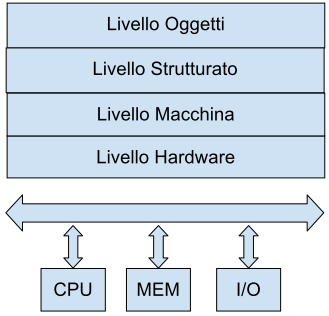
\includegraphics[scale=1]{figures/hwsw.png}
\caption{Architettura hardware-software} 
\end{figure}
\end{center}

\subsection{Il software - Architettura a tre livelli}

Un software che utilizza una base di dati (data-centric application) può essere decomposto in tre parti: il \textbf{data layer} è il livello dove vengono salvati i dati (il database), il \textbf{business rule layer} è il livello logico del progetto, il \textbf{presentation layer} è il livello che permette di far interagire l’utente con l’applicazione (può essere un messaggio su schermo, un comando vocale, un’interfaccia a gesture, ecc…).  
Nella storia, il presentation layer si è evoluto con l’avanzare della tecnologia:

\begin{itemize}

\item quando si programmava utilizzando il linguaggio macchina, gli input erano le schede perforate e i nastri magnetici;
\item con il linguaggio assemblativo sono stati introdotti i primi comandi a riga di comando (con l’introduzione dei monitor);
\item con l’evoluzione a livello strutturato si è arrivati al concetto di WIMP (windows, icons, menus, pointers) che ha rivoluzionato l’utilizzo dei calcolatori;
\item infine si ha l’evoluzione della WIMP in GUI (Graphic User Interface), l’introduzione delle gesture, delle interfacce vocali e delle percezioni aptiche. 

\end{itemize}

\begin{center}
\begin{figure}[H]
\centering
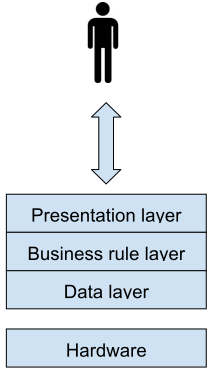
\includegraphics[scale=1]{figures/tla.png}
\caption{Architettura software a tre livelli} 
\end{figure}
\end{center}

\begin{flushright}Emanuele Costa Cesari\\Paolo Panarese\\29/09/2016\end{flushright}

\section{Modellazione dei dati}

Argomento centrale della lezione: \textbf{MODELLAZIONE DEI DATI}. Ripartiamo brevemente da ciò che nelle scorse lezioni abbiamo chiamato scenario ingegneristico della progettazione. Impareremo a costruire tre tipi di modelli: modello concettuale, modello logico e modello fisico. Ricordiamo qual è il ruolo di ognuno di essi.  

\begin{center}
\begin{figure}[H]
\centering
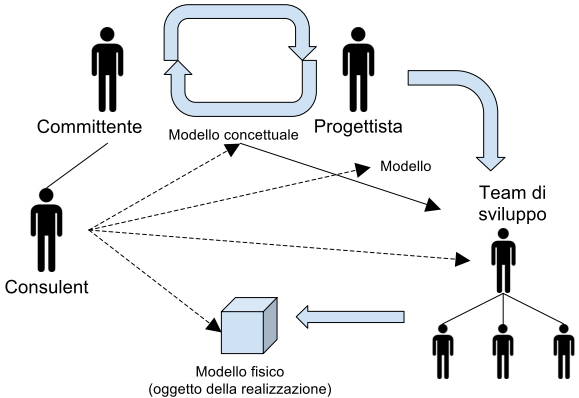
\includegraphics[scale=1]{figures/mdlng2.png}
\caption{Scenario della Progettazione} 
\end{figure}
\end{center}

Lo scenario tipico del progetto ingegneristico è il seguente: un \textbf{committente} che richiede un \textbf{prodotto} (nel caso dell’ingegneria informatica, un’applicazione), si rivolge ad un \textbf{progettista} che estrae i goal del progetto, i requisiti, i vincoli di qualità, tempo e costo e i test da effettuare. Il progettista produce per il committente un documento, chiamato \textbf{modello concettuale} che conterrà la stima dei costi e del risultato finale del prodotto (nel caso di progetti legati al mondo dell’informatica, spesso corrisponde al mockup). Il progettista raffina il modello concettuale creando un altro documento, il \textbf{modello logico} (che ha finalità più tecniche, contiene calcoli e specifiche tecniche). Modello concettuale e modello logico saranno la base da cui partiranno i membri del \textbf{team di sviluppo} (organizzato tipicamente in forma gerarchica, composta da un team leader e dagli sviluppatori) per trasformare queste informazioni nell’\textbf{oggetto della realizzazione} (nell’ingegneria informatica corrisponde con il modello fisico). Il committente, per assicurarsi che il lavoro sia corretto e con un buon rapporto qualità-prezzo, si affida ad una terza figura, il \textbf{consulente} che ha la responsabilità di supervisionare e verificare ogni fase del progetto.  È importante tenere presente che il progettista deve essere abile a presentare e mettere a confronto diverse soluzioni per il medesimo problema. Ogni soluzione deve specializzare un aspetto in particolare, perché committenti diversi potrebbero essere interessati a diversi aspetti dello stesso problema e magari vorranno porre enfasi su uno di questi. Un buon progettista deve saper dare una direzione alle idee, impostare una strategia di risoluzione. In qualità di ingegneri, dobbiamo essere in grado di creare modelli, di progettare una soluzione sia dal punto di vista visuale, che tecnico, che quantitativo. Per disegnare e particolareggiare ogni aspetto della modellazione ci si avvale di un insieme di strumenti. Un esempio nel caso di modellazione di software è UML, che è una raccolta di diversi tipi di diagrammi, ognuno dei quali aiuta il progettista a descrivere un particolare aspetto di ciò che deve realizzare. Per progettare sono quindi necessarie diverse abilità, perché bisogna modellare diversi aspetti. Nell’ambito dell’ICT distinguiamo tre aspetti principali:

\begin{itemize}

\item Hardware (ex. processor, display, elementi di networking, ecc.);
\item Software (ex. sistema operativo, software applicativo, driver, ecc.);
\item Dati: Un progetto non è ben progettato se non vengono considerati tutti e tre gli aspetti sopra elencati.

\end{itemize}

Un progetto non è ben progettato se non vengono considerati tutti e tre gli aspetti sopra elencati. 

\subsection{ESEMPIO – APPLICAZIONE CLIENT-SERVER}

Nella figura sottostante è rappresentata la struttura hardware di un’applicazione Client-Server: c’è un client connesso a Internet attraverso un ISP e un dispositivo chiamato Google Server. Queste due macchine sono collegate dal punto di vista hardware da una rete, basata su tecnologie come TCP/IP. Quello hardware non è l’unico livello da considerare, bisogna occuparsi anche della parte software. Infatti un dispositivo avrà bisogno di un sistema operativo e di applicazioni. 

\newpage
\begin{center}
\begin{figure}[H]
\centering
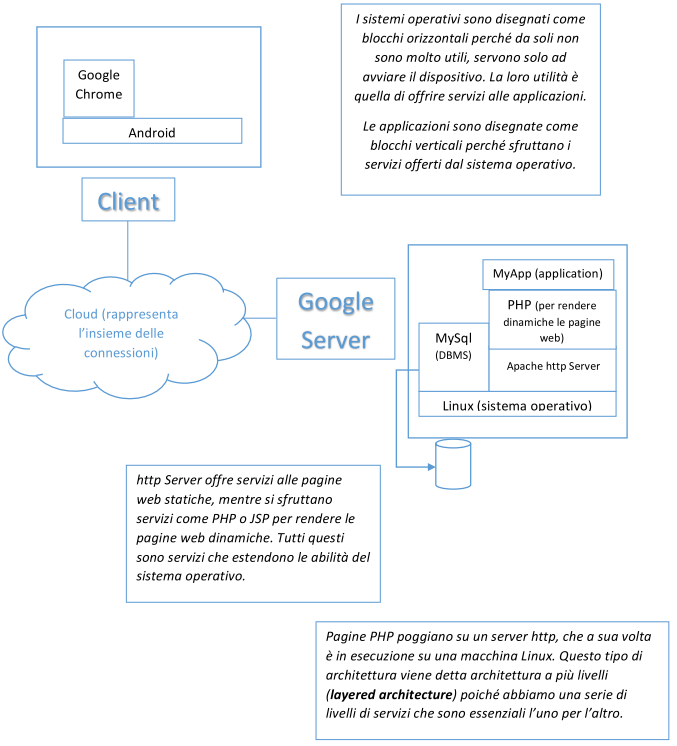
\includegraphics[scale=0.8]{figures/google_cs.png}
\caption{Scenario Google Client-Server} 
\end{figure}
\end{center}
\newpage

Il Server Hardware è una macchina destinata a soddisfare richieste. Quando si disegna l’architettura software si progetta il tipo di software da inserire nella macchina hardware e le richieste che potranno essere realizzate. Infine, bisogna progettare anche un’architettura dati.  
Oggi disegneremo la nostra prima Data Architecture. Come fare?  In generale quando parliamo di Software Engineering, le architetture sono disegnate in termini di classi. Ogni classe è specificata da un nome, degli attributi e dei metodi. Le classi possono interagire tra loro ed esistono diversi tipi di relazioni tra di esse: una classe può utilizzare un’altra classe, aggregarla, specializzarla, ecc.  Il problema sorge quando bisogna mappare queste classi in Data Structures per gestire la persistenza e la serializzazione dei dati.  Si dice che un’applicazione è in grado di gestire la persistenza dei dati se questi sopravvivono a diverse sessioni di utilizzo dell’applicazione.  Dare alle classi la possibilità di realizzare la persistenza dei dati non è sufficiente, poiché si ha anche la necessità di lavorare con essi. Normalmente facciamo utilizzo di database non solo per memorizzare dati, ma anche per recuperarli in un ordine differente da quello utilizzato per memorizzarli.  Abbiamo bisogno di eseguire diverse operazioni sui dati: crearli, cancellarli, modificarli, trasformarli, ecc. Per fare questo utilizziamo delle funzioni di alto livello, come le Associative Functions.  Riscrivere queste funzioni ogni volta che scriviamo un programma è molto dispendioso e poco pratico. Perciò si utilizza un \textbf{DBMS} (\textbf{DataBase Management System}) come MySql, un software orientato al data processing, che rappresenta i dati in maniera differente. Un DBMS organizza in “librerie” le funzioni di cui abbiamo bisogno per l’elaborazione dei dati. Utilizzare le funzioni di alto livello fornite da un DBMS rende il nostro codice più efficiente e la programmazione più veloce e meno costosa. Quindi non è necessario che le nostre classi gestiscano direttamente la persistenza e implementino funzioni di ricerca, perché abbiamo a disposizione del software specifico che si occupa della gestione dei dati. Non scriveremo codice in termini di Object Oriented code, ma faremo quello che è chiamato \textbf{ORM} (\textbf{Object Relational Mapping}). Un esempio di Object Relational Mapper è Hibernate. Per esempio, possiamo scrivere un programma Java che richiede dati ad un database relazionale. Un ORM come Hibernate si occupa di trasformare le richieste delle classi Java in richieste al database, traducendo le operazioni sugli Oggetti in operazioni su Tabelle del database. La progettazione di un’applicazione richiede la realizzazione di questi passi:

\begin{itemize}

\item Goal;
\item Requisiti;
\item Architettura Sw, Architettura Hw, Architettura dati;
\item Test e deployment;
\item Operation

\end{itemize}


\subsection{ESEMPIO}

Iniziamo	a	vedere	come	modellare	concettualmente	i	dati.	Data	una	situazione	come	quella	descritta	dall’Entity	Relationship	Diagram	in	figura,	un	ingegnere	deve	essere	in	grado	di	immaginare	come	sarà	il	software.	

\begin{comment}
\centering
%\scalebox{.87}{
\begin{tikzpicture}[node distance=5cm, every edge/.style={link}]

\node[entity] (cus) {Customer};
\node[attribute] (name) [below of=cus] {Name} edge (cus);
\node[attribute] (addr) [below right of=cus] {Address} edge (cus);
\node[attribute] (bdat) [below left of=cus] {B\_Date} edge (cus);
\node[attribute] (fdat) [left of=bdat] {F\_Date} edge (cus);

\node[relationship] (buys) [right of=cus] {Buys} edge(cus);
\node[attribute] (dat) [below of=buys] {Date} edge(buys);
\node[attribute] (qnt) [below right of=buys] {Quantity} edge(buys);
\node[attribute] (spr) [below left of=buys] {Selling price} edge(buys);

\node[entity] (prod) [right of=buys] {Product} edge(buys);
\node[attribute] (pc) [below of=prod] {PC} edge(prod);
\node[attribute] (pnam) [below right of=pc] {Name} edge(prod);
\node[attribute] (ppic) [below left of=prod] {Picture} edge(prod);
\node[attribute] (desc) [right of=pnam] {Description} edge(prod);
\node[attribute] (lprc) [left of=ppic] {List price} edge(prod);

\end{tikzpicture}
%}
\end{comment}

\begin{center}
\begin{figure}[H]
\centering
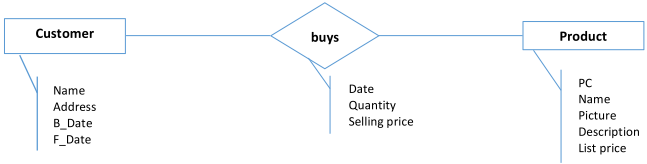
\includegraphics[scale=0.8]{figures/ERD.png}
\caption{Entity Relationship Diagram} 
\end{figure}
\end{center}

\textbf{Customer} e	\textbf{Product} prendono	il	nome	di	entità,	poiché	possono	esistere	anche	da	sole,	sono	definite	senza	dipendere	dagli	altri	elementi	del	database. \textbf{Buys} è	una	\underline{\textit{\textbf{relazione}}}	e	non	può	esistere	da	sola,	dal	momento	che	non	avrebbe	alcun	significato	se	posta	fuori	da	un	contesto	(esempio:	non	posso	definire	un	acquisto	senza	indicare	l’acquirente	e	il	prodotto	acquistato).	Possiamo	rappresentare	un	database	come	un	grafo,	in	cui	ogni	\textbf{Entità}	è	un	nodo	e	ogni	\textbf{Relazione}	è	un	arco.	Su	questo	grafo	possiamo	individuare	diversi	percorsi,	che	corrispondono	a	interrogazioni	al	database	(query).

\subsection{ESEMPIO - THE COMPANY DATABASE}

Facciamo	un	passo	in	avanti	analizzando	qualcosa	di	più	complesso.	Consideriamo	l’esempio	\textit{The	Company	Database} del	libro	di	testo.	

\begin{center}
\begin{figure}[H]
\centering
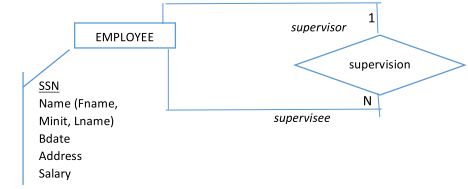
\includegraphics[scale=1]{figures/tcd.png}
\caption{The Company Database} 
\end{figure}
\end{center}

Notiamo	che:

\begin{itemize}

\item L’attributo	SSN	dell’entità	employee	è	sottolineato.	Con	la	sottolineatura	si	indica	la	\textbf{chiave	primaria},	ovvero	l’attributo	(o	l’insieme	di	attributi)	che	identifica	univocamente	un’istanza	di	una	certa	entità.	Non	potranno	esistere	due	employees	aventi	attributo	SSN	con	lo	stesso	valore;
\item I	numeri	indicano	la	\textbf{cardinalità}	della	relazione.	Nell’esempio	abbiamo	che	un	employee	può	supervisionare	N	employees	ed	un	employee	può	essere	supervisionato	da	un	solo	employee	(relazione	uno-a-molti).

\end{itemize}

Espandiamo	lo	schema	precedente,	aggiungendo	altre entità...

\newpage
\begin{center}
\begin{figure}[H]
\centering
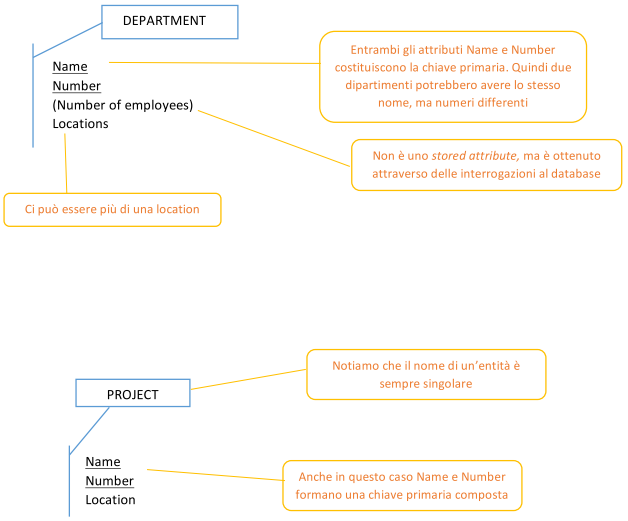
\includegraphics[scale=0.8]{figures/tcdBIG.png}
\caption{The Company Database} 
\end{figure}
\end{center}
\newpage

... e	le	relazioni	che	intercorrono	tra	di	esse:

\begin{center}
\begin{figure}[H]
\centering
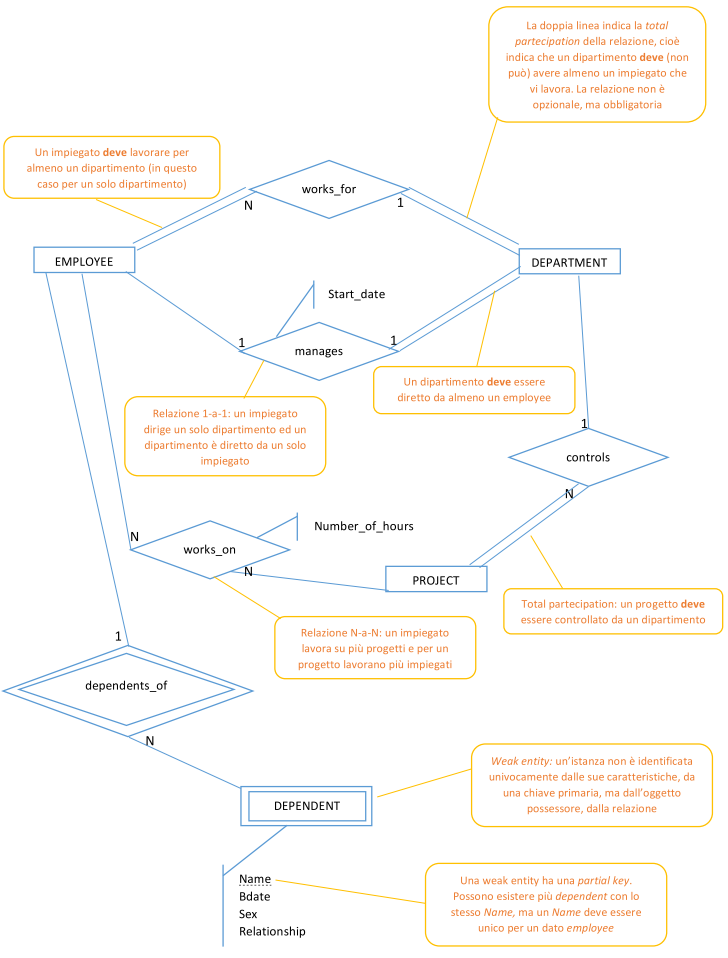
\includegraphics[scale=0.8]{figures/tcdBIG2.png}
\caption{The Company Database 2} 
\end{figure}
\end{center}

\begin{flushright}Floriana Accoto\\Emanuele Trono\\05/10/2016\end{flushright}


\section{Conceptual Model}

Nella lezione precedente abbiamo visto come realizzare il data modeling, composto da CM (Conceptual model), LM (Logical model), FM (Physical model). 
Gli elementi principali del CM sono tre: Entity type, Relation type, Attributes.

\begin{center}
\begin{figure}[H]
\centering
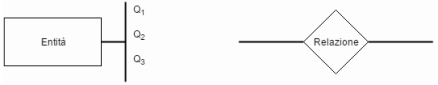
\includegraphics[scale=1]{figures/ER.png}
\caption{Elementi CM} 
\end{figure}
\end{center}

Combinando questi elementi si crea il CM. Naturalmente esistono delle regole e dei vincoli da rispettare, in quanto si sta parlando di un linguaggio formale. Ad esempio non sono consentite operazioni del genere:

\begin{center}
\begin{figure}[H]
\centering
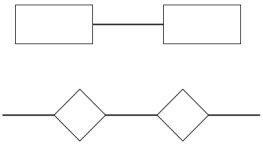
\includegraphics[scale=1]{figures/ERcomb.png}
\caption{Operazioni proibite in un ER} 
\end{figure}
\end{center}

vale a dire non è possibile collegare direttamente due entità o due relazioni. 

La logica da seguire è la seguente,

\begin{center}
\begin{figure}[H]
\centering
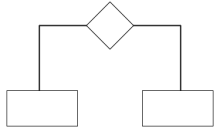
\includegraphics[scale=1]{figures/correctER.png}
\caption{ER corretto} 
\end{figure}
\end{center}

tenendo conto che le entità devono avere necessariamente degli attributi, mentre le relazioni possono anche non averne. 

Il modello concettuale fornisce anche i seguenti vincoli:

\begin{itemize}

\item Cardinalità;
\item Total Participation;
\item Primary Key.

\end{itemize}

Per ogni entità partecipante ad una relazione viene specificata una cardinalità di relazione. Essa è una coppia di numeri naturali che specifica il numero minimo e massimo di istanze di relazione a cui un’istanza dell'entità può partecipare. Esistono tre tipi di cardinalità: 

\begin{itemize}

\item 1 a 1;
\item 1 a molti;
\item Molti a molti.

\end{itemize}

Nell’ultimo caso conviene mettere due lettere differenti perché riportare la stessa lettera (ad esempio n to n) fa capire che le entità possiedono lo stesso numero di partecipanti, ma questo è errato. Infatti non si è in 
grado di prevedere a priori il numero esatto dei partecipanti, portando il progettista a fornire un’informazione errata del modello. 

Vediamo degli esempi, per comprendere meglio come differenziare i vari tipi di cardinalità: 

\begin{itemize}

\item

\begin{center}
\begin{figure}[H]
\centering
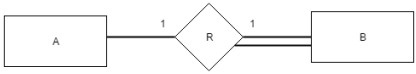
\includegraphics[scale=1]{figures/ER11.png}
\caption{Relazione 1 a 1 $\rightarrow$ A (person) - R(has) – B (Driving license)} 
\end{figure}
\end{center}

La patente è un’entità che esiste anche se non ha un possessore, così come la persona, ed ha come attributi numero, ente, data di rilascio, ecc. In questo caso ha senso parlare di totally partecipation solo nel caso della patente, che non può non essere associata ad una persona. Mentre la persona non deve necessariamente avere una patente e potrebbe avere come attributi il nome, cognome, codice fiscale. 
N.B. Un esempio errato è quello di definire come entità il codice fiscale di una persona. Infatti ogni individuo possiede un codice fiscale che lo caratterizza, ma il codice fiscale è un’attributo dell’entità persona, in quanto è una caratteristica della persona. Inoltre possiamo affermare che il codice fiscale è un autonomous entity type.

\item{}

\begin{center}
\begin{figure}[H]
\centering
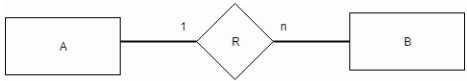
\includegraphics[scale=1]{figures/ER1n.png}
\caption{Relazione 1 a molti $\rightarrow$ A (Person) – R (Own) – B (Car)} 
\end{figure}
\end{center}

È una relazione uno a molti poiché una persona può possedere più macchine, al contrario una macchina non può essere posseduta da più persone. Di conseguenza, in questo caso, non si può parlare di total participation, perché una persona può non avere un’auto e un’auto può non avere un proprietario.

\item{}

\begin{center}
\begin{figure}[H]
\centering
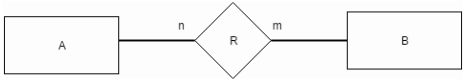
\includegraphics[scale=1]{figures/ERnm.png}
\caption{Relazione molti a molti $\rightarrow$ A (Car) – R (Has) – B (Optional)} 
\end{figure}
\end{center}

Questo tipo di relazione ci permette di introdurre il concetto di pattern, di cui si parla nell’appendice. 

\end{itemize}

\subsection{Il valore NULL}

Il valore NULL è un valore speciale in un DB, infatti la PK (chiave primaria), cioè un singolo raggruppamento di attributi dell’entità che ci permette di identificare univocamente un’istanza dell’entità stessa, deve essere necessariamente di tipo NOT NULL, vediamo il perché.  
È buona norma evitare di inserire valori di tipo NULL all’interno del DB, in quanto sono indice di mancanza di informazioni e al momento dell’estrazione dei dati, non si potrà comprendere se il dato non è stato inserito, se non se ne conosce il valore, se c’è stato un errore in fase di inserimento ecc. 
Pertanto la presenza di valori di tipo NULL significa che non solo non si conosce il valore di un determinato attributo, ma non si sa neanche il motivo per cui quel valore non è presente.  
La maniera corretta di inserire in un DB devi valori nulli è quella di inserire delle stringhe vuote. Ad esempio se si vuole inserire in un record una persona che non ha un secondo nome, mentre tra gli attributi dell’entità persona compare, il modo corretto di procedere è quello di inserire una stringa vuota, cioè “”. 
ESEMPIO: Se si volesse calcolare l’età media di un gruppo di persone inserite in un DB, è sufficiente che ci sia un unico campo in cui compaia un valore di tipo NULL per fare non essere in grado di calcolarla. In quel caso si potrà avere solo una stima dell’età media, ma non l’età media esatta.

\[
	3 + 2 + NULL = NULL
\]

\subsection{ANALIST}

\begin{center}
\begin{figure}[H]
\centering
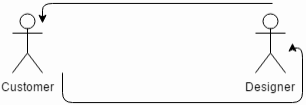
\includegraphics[scale=1]{figures/custdes.png}
\caption{Customer \& Designer} 
\end{figure}
\end{center}

\subsection{SCHEMA}

\begin{center}
\begin{figure}[H]
\centering
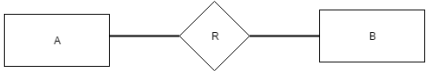
\includegraphics[scale=1]{figures/ERschema.png}
\caption{Schema ER} 
\end{figure}
\end{center}

È importante capire che gli schemi di database usati nei precedenti esempi forniscono una INTENTIONAL DESCRIPTION OF DATABASE, cioè, mediante l’uso di un linguaggio formale si è in grado di fornire una descrizione logica del database. Si useranno ora nuovi elementi che portano a fornire una EXTENSIONAL DESCRIPTION OF DATABASE. Rientrano in questa categoria: 

\begin{itemize}

\item Tabelle;
\item Entity Set.

\end{itemize}

Le tabelle in un database relazionale sono un insieme di elementi che sfruttano un modello in cui ci sono colonne verticali (ogni colonna è identificata con il nome di un attributo) e righe orizzontali, dove la cella del database rappresenta il punto in cui colonna e riga si intersecano. Ogni tabella del database coincide con l’entità presa in analisi, dove le colonne rappresentano gli attributi. Se la quantità degli attributi ha un valore fissato, le righe invece hanno un valore variabile in quanto rappresentano il numero di istanze contenute 
nell’entità. La riga di una tabella prende il nome di record della tabella. Le tabelle sono alla base delle relazioni. 
Un altro tipo di EXTENSIONAL DESCRIPTION OF DATABASE non si basa sull’uso delle tabelle ma sulla SET THEORY. Per poter fornire la definizione di entity set, bisogna definire che cos’è un entity type. Un entity type definisce una collezione (o set) di entità che hanno gli stessi attributi. Ogni entity type è descritto dal nome e dai suoi attributi. La collezione di tutte le entità di un particolare entity type nel database in qualsiasi punto nel tempo è chiamato entity set o entity collection.

\begin{center}
\begin{figure}[H]
\centering
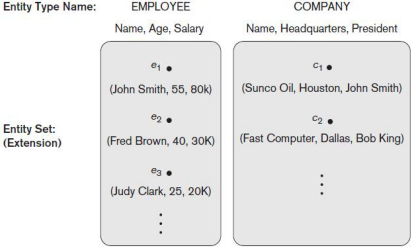
\includegraphics[scale=1]{figures/entity_set.png}
\caption{Entity Set} 
\end{figure}
\end{center}

L’obiettivo che ci si pone è quello di usare uno stesso DB per soddisfare più bisogni.  
ES. Una catena di negozi, che ha sedi diverse, utilizza copie dello stesso DB per registrare gli acquisti degli utenti. Naturalmente viene usata una copia dello stesso DB in ogni sede e ovviamente gli acquisti registrati saranno differenti in ogni sede.

\begin{center}
\begin{figure}[H]
\centering
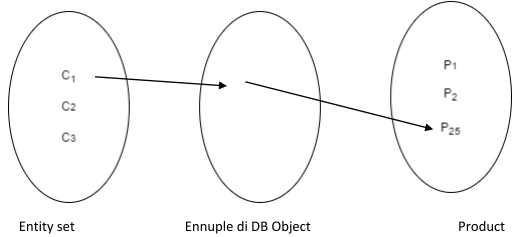
\includegraphics[scale=1]{figures/entity_setEV.png}
\caption{Entity Set Eulero-Venn} 
\end{figure}
\end{center}

La precedente descrizione del modello è stata estrapolata dal libro “Fundamentals of database systems”, mentre a lezione l’esempio si basava sulle entità Venditore e Prodotto. Il legame tra un’istanza di product e una di customer mi permette di ottenere una relazione che prende il nome di Tuple o ennupla. La tupla è una lista finita ordinata di elementi. Gli elementi di una tupla sono contenuti all’interno di “()”, ed ogni elemento 
è separata da una ”,”. Si comprende facilmente che gli elementi di una tupla sono gli attributi dell’entità presa in considerazione. Quindi, una relazione è un set di tuple degli oggetti del database. 
Gli attributi che hanno il ruolo di caratterizzare le entità e le relazioni possono essere definiti concettualmente:

\begin{itemize}

\item semplici;
\item composti;
\item multipli;
\item multipli \& composti.

\end{itemize}

Un attributo è semplice quando fornisce una singola informazione di base che caratterizza l’entità, assumendo un singolo valore (professione di una persona). Un attributo è composto quando è creato tramite l’uso di attributi semplici (l’indirizzo è composto dal tipo di via, nome della via, indirizzo civico, paese). Un attributo si dice multiplo quando a esso possono essere associati più valori dello stesso tipo contemporaneamente (locazione nel caso di un dipartimento universitario). Un esempio di attributo multiplo e composto è il numero di telefono, il quale è composto dal prefisso e dal numero. Durante la creazione di un database, tutti gli attributi composti e multipli devono essere convertiti in attributi semplici perché nei database relazionali sono accettati solo gli attributi semplici. 


\subsection{Come iniziare la progettazione di un DB}

Si parte con carta e penna, realizzando uno schema, non necessariamente corretto, in base alle richieste del committente. Solitamente non si riesce a creare un DB corretto subito. Vediamo un esempio.  
Il modello in figura evolve dinamicamente per ogni soluzione migliore che si riesce a trovare. 
Si è notato, in questo caso, che era più opportuno non considerare il nome del manager e la data di inizio del suo lavoro come attributo dell’entità department, ma creare una nuova entità di tipo impiegato che è in relazione con department.

\begin{center}
\begin{figure}[H]
\centering
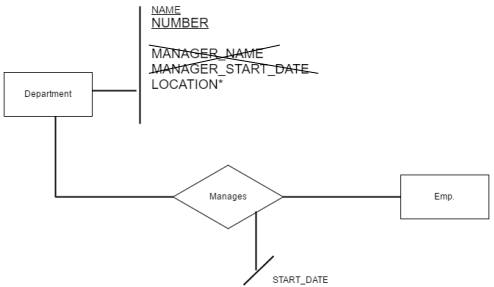
\includegraphics[scale=1]{figures/incER.png}
\caption{Incremental ER} 
\end{figure}
\end{center}

\subsection{Ternary relation type}

\begin{center}
\begin{figure}[H]
\centering
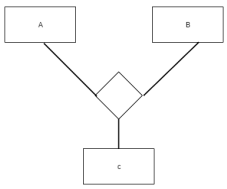
\includegraphics[scale=1]{figures/tER.png}
\caption{Ternary Relationship} 
\end{figure}
\end{center}

Nel caso in cui si ha la presenza di tre entità, in funzione della relazione usata, siamo in grado di estrapolare delle informazioni più precise. Per farlo si sfrutta una relazione ternaria, che diversamente da quella binaria, mette in collegamento attraverso una singola relazione tre entità. Le informazioni ottenute da una relazione ternaria contengono informazioni più precise rispetto a quando vengono usate delle relazioni binarie. Possiamo esprimere la precedente affermazione tramite disuguaglianza matematica: 

\[
	TernaryRelationship > BinaryRelationship
\]

\begin{center}
\begin{figure}[H]
\centering
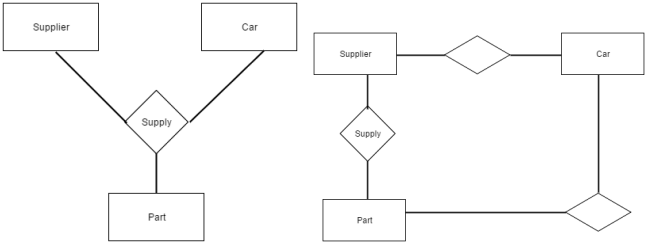
\includegraphics[scale=0.8]{figures/tER2.png}
\caption{Ternary Relationship and Three Binary Relationship} 
\end{figure}
\end{center}

Gli schemi rappresentati in figura sono equivalenti. Solo che, come già detto, 3 relazioni binarie contengono meno informazioni di una relazione ternaria. 
Per mantenere la stessa quantità di informazioni si fa uso della REIFICAZIONE, che consiste nel trasformare una relazione in un’entità. In questo modo si ha la presenza delle tre entità, un’entità reificata e tre relazioni binarie che collegano le entità all’entità reificata.  
Quindi continuo ad usare relazioni binarie anziché utilizzare relazioni ternarie, senza perdere informazione. 
In questo modo l’informazione estrapolata dalla relazione ternaria e l’informazione estrapolata dalla procedura di reieficazione è equivalente: 

\[
	TernaryRelationship := 3\ BinaryRelationShip + 1\ Entity Type
\]

L’uso di questa procedura è a discrezione esclusivamente del dal progettista. 

\begin{center}
\begin{figure}[H]
\centering
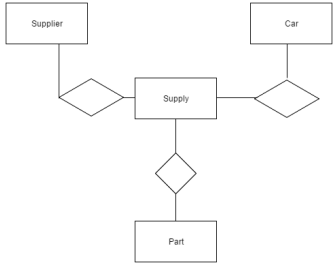
\includegraphics[scale=1]{figures/reification.png}
\caption{Reification of a Ternary Relationship} 
\end{figure}
\end{center}


\section{APPENDICE}

\subsection{DESIGN PATTERN}

Anche per i db esistono dei design pattern.

\begin{itemize}

\item{\textbf{\underline{X toX (es. Object type of object)}}} $\rightarrow$ Consiste nella distinzione tra oggetti unici, cioè rappresentati da un codice identificativo (automobile, armi, ...), e oggetti che sono istanze dello stesso tipo assolutamente identiche (capi di abbigliamento, generi alimentari, ...). Quindi la differenza consiste nel fatto che, si può acquistare, ad esempio, un’istanza di un oggetto (pacco di pasta) e non il singolo oggetto oppure il singolo oggetto se identificabile univocamente con qualche criterio. 
Questo pattern è utile in quanto è un tipico errore quello di inserire, all’interno del db, un oggetto al posto del tipo di oggetto.

\item{\textbf{\underline{Temporal Dimension}}} $\rightarrow$ Prima di dire lo scopo dell’utilizzo di questo pattern, è di fondamentale importanza rimarcare un concetto da tenere a mente quando si ha a che fare con il mondo dei DB, cioè che i dati sono fondamentali, sono importanti, sono una risorsa preziosa e a meno di casi eccezionali non vanno eliminati dal DB perché potrebbero ritornare utili in qualsiasi momento. Si sta facendo riferimento al concetto di Data Mining. ES. Se si dovessero perdere i dati (risorse immateriali) di una DB di una banca, che è un ente composto da risorse umane, materiali e immateriali, comporterebbe la perdita di tutte le informazioni relative ai correntisti o ai titoli bancari, di conseguenza le risorse materiali non avrebbero un possessore.  
Detto ciò, passiamo ad un esempio pratico per comprendere l’utilizzo di questo pattern.  Come si può vedere nella figura sottostante, il pattern Temporal Dimension esprime il fatto che alcuni attributi possano variare nel tempo, pertanto alle volte si ritiene opportuno avere uno storico delle informazioni, nel nostro caso variazioni di dati riguardanti il proprietario o 
l’automobile. In altre parole, sto aggiungendo la dimensione temporale al mio DB, per avere traccia delle varie versioni di un dato oggetto.   

\end{itemize}

\begin{center}
\begin{figure}[H]
\centering
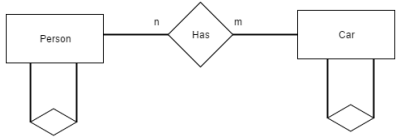
\includegraphics[scale=1]{figures/tdim.png}
\caption{Temporal Dimension} 
\end{figure}
\end{center}

\begin{flushright}Cristian Annicchiarico\\Mattia Marzano\\06/10/2016\end{flushright}


\section{Esercizio - Fermate Autobus}

I diagrammi Entità-Relazione (ER) sono stati estesi e migliorati con lo scopo di includere tecniche di modellazione tipiche del design object-oriented. Il risultato è una nuova classe di diagrammi definiti EER (Extended Entity-Relationship), che si avvicinano di più al concetto di diagramma delle classi UML. 

\textbf{Esercizio}: Siamo una compagnia di bus e vogliamo un’architettura del DB che ci aiuti a gestire il nostro business. Dobbiamo prendere in considerazione i seguenti punti:

\begin{itemize}

\item Bus;
\item Linee (fermate, collegamenti);
\item Impiegati;
\item Viaggiatori;
\item Biglietti (settimanali, mensili, annuali).

\end{itemize}

Gli aspetti precedenti sono ciò che chiamiamo \textbf{requisiti}, che il nostro progetto deve soddisfare. Alcune assunzioni aggiuntive verranno considerate nel prosieguo dell’esercizio in modo da ridurre la complessità del progetto. Senza perdita di generalità, considereremo solamente biglietti che sono validi in un lasso di tempo maggiore di 1 giorno (ovvero, settimanali/mensili/annuali), poiché i biglietti giornalieri non ci permettono di avere dettagli su chi stia usando quel biglietto, mentre, ad esempio, i biglietti settimanali richiedono una sorta di tessera che contiene i dati personali del viaggiatore. 

\textbf{Importante}: dobbiamo sempre ricordare che vogliamo un’architettura dei dati che soddisfi le esigenze di tutti i nostri stakeholder. In altre parole, il nostro design pattern è: Un database, multiple applicazioni (ovvero, interfacce e presentazioni differenti per gli stessi dati: vedi Figura 1). Anche se il database è lo stesso, utenti diversi usufruiscono di viste differenti degli stessi dati. Per spiegarlo attraverso un esempio, prendete un qualsiasi gioco di carte da tavolo: il database è “tutte le carte sul tavolo”, mentre ogni utente percepisce una diversa presentazione (infatti, lui o lei può solo sapere quali carte scoperte sono poste sul tavolo, quali carte sono nella sua mano, e quali carte erano nella sua mano).   

\begin{center}
\begin{figure}[H]
\centering
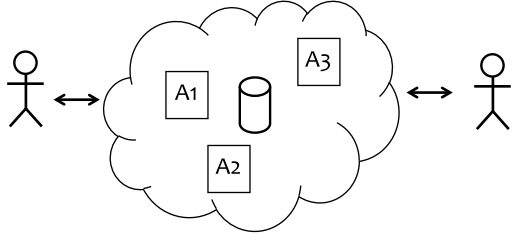
\includegraphics[scale=1]{figures/1DBmAPP.png}
\caption{Un database, multiple applicazioni} 
\end{figure}
\end{center}

Al fine di svolgere l’esercizio, consideriamo separatamente I requisiti. Prima di tutto, consideriamo le entità “Traveller” ed “Employee”. Al momento, modelliamole entrambe come un’unica entità “Person” con gli attributi appropriati:

\begin{center}
\begin{figure}[H]
\centering
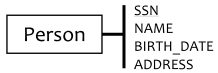
\includegraphics[scale=1]{figures/person_entity.png}
\caption{Entità "Person"} 
\end{figure}
\end{center}

Consideriamo ora linee con fermate e collegamenti. Questo ci porta alla creazione dell’entità “Line” (Figura 3).

\begin{itemize}

\item{\textbf{Domanda}}: dovremmo modellare le fermate di una certa linea come un attributo multiplo?
\item{\textbf{Risposta}}: No, poiché se consideriamo una fermata interposta tra due linee, dovremmo dichiararla due volte nel nostro database (ovvero, come un attributo sia della prima che della seconda linea). Questo violerebbe la terza regola dei database.

\end{itemize}

\textbf{Terza regola dei database}: Mai aggiungere ridondanza al vostro database! 

\textbf{Anticipazione}: In un diagramma E-R, la chiave primaria è solo concettuale (dobbiamo scegliere un campo che sia unico). Nella pratica, quando traduciamo un diagramma E-R nel suo corrispondente modello relazionale (modello logico), aggiungeremo un campo ID, responsabile dell’unicità di ciascuna entry nelle nostre tabelle. Esso sarà la nostra chiave primaria, ma non è visibile agli utenti. 

\begin{center}
\begin{figure}[H]
\centering
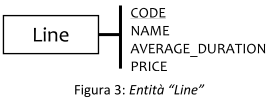
\includegraphics[scale=1]{figures/line_entity.png}
\caption{Entità "Line"} 
\end{figure}
\end{center}

Come specificare quali fermate attraversa una linea? Prima di tutto, dobbiamo modellare le fermate. Lo facciamo tramite un’entità “Stop”. 

\begin{center}
\begin{figure}[H]
\centering
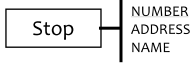
\includegraphics[scale=1]{figures/stop_entity.png}
\caption{Entità "Line"} 
\end{figure}
\end{center}

Come modellare i collegamenti tra le fermate? Abbiamo considerato varie alternative. Esaminiamole in ordine. 

\begin{itemize}

\item{\textbf{Prima alternativa per modellare le fermate}}

Poiché una linea è una sequenza di fermate, può essere considerata come una coda. Nei database, una coda può essere modellata creando una relazione ricorsiva (Figura 5). Comunque, questo approccio ha un problema. Prendete come esempio la Figura 6, in cui consideriamo due linee (rossa e verde). Nella linea rossa, la fermata blu è la numero 2, mentre nella linea verde, la fermata blu è la numero 3. Dovremmo modellare la fermata blu come la seconda o la terza fermata della coda? La risposta è: nessuna delle due, poiché la fermata blu deve comportarsi come terza fermata della coda per la linea rossa e come seconda fermata della coda per la linea verde. Con una simile architettura del database, come possiamo tenere traccia di quale fermata è situata a un certo punto di una certa linea? 

\begin{center}
\begin{figure}[H]
\centering
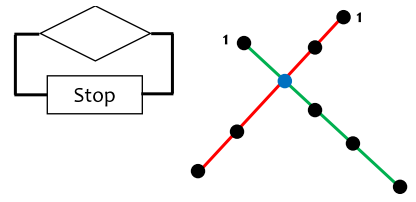
\includegraphics[scale=1]{figures/queue_stop.png}
\caption{A sx: Modellare una coda (prima alternativa), dx: Due line che condividono la stessa fermata} 
\end{figure}
\end{center}

\item{\textbf{Seconda alternative per modellare le fermate}}

Poiché il problema con la precedente soluzione era la mancanza di un collegamento tra la coda di fermate e le linee, un’idea sarebbe rimodellare lo scenario come mostrato in figura successiva. Comunque, questa architettura evidenzia due problemi: 

\begin{itemize}

\item E’ troppo complessa. Un requisito banale (una coda) non dovrebbe creare una grande complessità nel diagramma;
\item La relazione 1-1 tra “Queue” e “Line”, insieme con la totale partecipazione su entrambi i lati della relazione 1-1, suggerisce che di fatto “Queue” e “Line” siano lo stesso oggetto. Quindi, potremmo comprimerle in un’unica entità.   

\end{itemize}

\begin{center}
\begin{figure}[H]
\centering
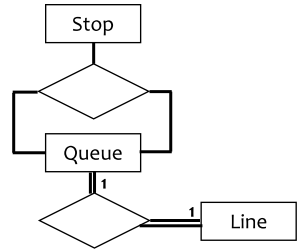
\includegraphics[scale=1]{figures/queue.png}
\caption{Modellare una coda (seconda alternativa)} 
\end{figure}
\end{center}

\item{\textbf{Terza alternative per modellare le fermate (la migliore)}}

Dopo tali considerazioni, abbiamo finito per semplificare la nostra architettura. La migliore alternativa (finora) è avere una semplice relazione N a M tra “Line” e “Stop” con un attributo \#Step che consente la creazione di una lista ordinata. E’ stato aggiunto un attributo addizionale Minutes, per modellare il tempo necessario, a partire dall’inizio di una corsa, per attraversare quella fermata. Inoltre, è un attributo multiplo, che dunque consente varie tempistiche per diverse ore della giornata. Lo scenario è riassunto nella successiva figura. Questa soluzione ha vari benefici:

\begin{itemize}

\item La complessità della ridefinizione della lista è spostata dentro all’applicazione. Quando una fermata è rimossa da una linea, deve essere eseguito da parte dell’applicazione il controllo di coerenza della lista;
\item Ha il giusto livello di complessità in paragone ai requisiti specificati;
\item Consente a un utente interessato di conoscere in che momento una linea attraversa una fermata: è sufficiente aggiungere il numero di minuti a partire dalla partenza del bus. 

\end{itemize}

\begin{center}
\begin{figure}[H]
\centering
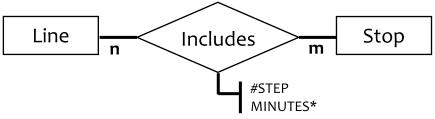
\includegraphics[scale=1]{figures/queue_final.png}
\caption{Modellare una coda (terza alternativa)} 
\end{figure}
\end{center}

\end{itemize}

Consideriamo ora il requisito dei biglietti. Non andremo a modellarlo come un’entità poiché significherebbe dire che i biglietti mensili esistono a prescindere dalla persona che li usa o a prescindere della linea per cui il biglietto è stato erogato. Questo ovviamente non è ciò che accade nella realtà. Motivo per cui modelleremo un biglietto come una relazione tra le entità interessate, come si può vedere dalla successiva figura. Questo è di fatto il modo più naturale di aggiungerlo nel nostro diagramma: un biglietto è un contratto, un pezzo di carta in cui sono scritte sia la persona che lo utilizza che la linea per cui può essere usato.

\begin{center}
\begin{figure}[H]
\centering
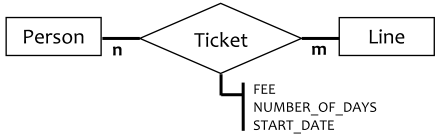
\includegraphics[scale=1]{figures/ticket_bus.png}
\caption{La relazione "Ticket"} 
\end{figure}
\end{center}

Infine, aggiungiamo il restante requisito al nostro diagramma: i bus. Prima di tutto, creiamo una nuova entità “Bus” (Prossima Figura). Abbiamo aggiunto alcuni attributi basilari, ma possiamo aggiungerne altri del tipo: numero di posti, se ha o meno supporto per persone disabili, se ha alcune utili agevolazioni per gli autisti, ecc..

\begin{center}
\begin{figure}[H]
\centering
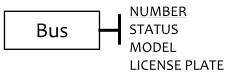
\includegraphics[scale=1]{figures/bus.png}
\caption{Entità "Bus"} 
\end{figure}
\end{center}

Ora dobbiamo analizzare due aspetti:

\begin{itemize}

\item Come modellare la tabella oraria per le linee?
\item Come tener traccia di quale bus ha servito una certa linea in un certo giorno a una certa ora?  

\end{itemize}

Per rispondere alla prima domanda, abbiamo introdotto l’entità “Race” (Successiva figura). Questa nuova entità debole modella una particolare istanza di una linea (con una tabella oraria). Mentre “Line” indica un percorso teorico attraverso alcune fermate, “Race” è una particolare istanza di “Line” che ha un orario di partenza formale per ogni giorno della settimana. 

\begin{center}
\begin{figure}[H]
\centering
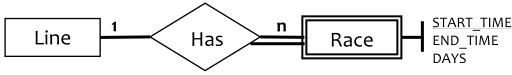
\includegraphics[scale=1]{figures/race_line.png}
\caption{Entità “Race” e suo collegamento all’entità “Line”} 
\end{figure}
\end{center}

Con questa nuova entità, la seconda domanda può essere riformulata nel seguente modo: come tener traccia di quale bus ha servito una certa corsa? Questo può essere banalmente ottenuto aggiungendo una relazione tra “Race” e “Bus” (Successiva figura). Il diagramma ER finale è riportato in Figura 13. Comunque, questa impostazione non considera chi ha guidato in una certa corsa. Non abbiamo esplorato questo punto nella lezione, ma può essere ottenuto in vari modi:

\begin{itemize}

\item Modificando la relazione “Served” in successiva figura in una relazione ternaria, in cui il terzo collegamento è attaccato all’entità “Person”;
\item Aggiungendo una relazione tra “Person” e “Race” (ma questo obbliga gli impiegati a guidare sempre nella stessa corsa e non permette modifiche negli assegnamenti).

\end{itemize}

\begin{center}
\begin{figure}[H]
\centering
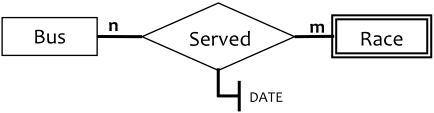
\includegraphics[scale=1]{figures/served.png}
\caption{La relazione “Served”} 
\end{figure}
\end{center}

\newpage
\begin{center}
\begin{figure}[H]
\centering
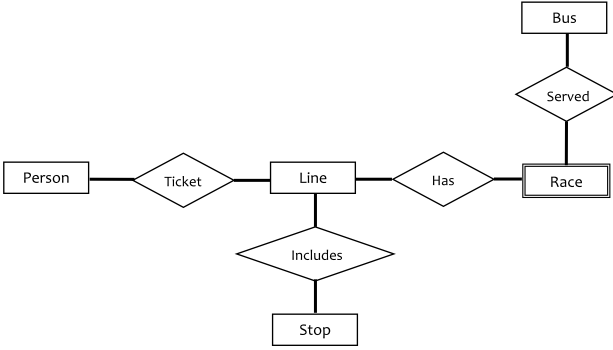
\includegraphics[scale=0.8]{figures/finalbusER.png}
\caption{Diagramma ER finale per l’esercizio sulla compagnia di bus} 
\end{figure}
\end{center}
\newpage

Le fermate dovrebbero essere collegate alle corse? Introduciamo un altro design pattern che risolve questo problema: il Preventivo Consuntivo. Questo ci consentirà di salvare l’informazione circa il tempo effettivo in cui una corsa ha attraversato una certa fermata in un certo giorno (permettendoci, ad esempio, di ricalcolare periodicamente il tempo di arrivo stimato sulla base delle statistiche).

\subsection{Design Pattern: Preventivo-Consuntivo}

Questo pattern gestisce la previsione di un evento e la sua effettiva realizzazione. Introduciamolo tramite un esempio: la prenotazione in un hotel. La previsione è la prenotazione di una camera, mentre la realizzazione è ciò che accade effettivamente (ovvero, se la camera viene occupata o meno al tempo previsto). In questo caso, possono accadere tre situazioni: 

\begin{itemize}

\item Qualcuno prenota la camera e la usa (prenotazione + uso);
\item Qualcuno prenota la camera ma non la usa (prenotazione + non uso);
\item Nessuno prenota la camera ma qualcuno la usa (no prenotazione + uso).

\end{itemize}

Di fatto possono accadere più situazioni (per esempio, vi potrebbero essere multiple prenotazioni e cancellazioni, o una prenotazione per N persone e $N \neq M$ persone che la usano, ecc…) Se il diagramma originario contiene una relazione tra due entità A e B (ad esempio “Person” e “Room”) che è di tipo Preventivo-Consuntivo (ad esempio “Books” e “Uses”), questo pattern richiede di dividere la relazione in due relazioni: prevenire (Books) e consumare (Uses). Questa situazione è illustrata nella successiva figura:

\begin{center}
\begin{figure}[H]
\centering
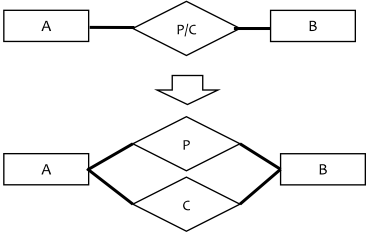
\includegraphics[scale=1]{figures/prevcon.png}
\caption{ Divisione della relazione. P e C stanno rispettivamente per Prevenire e Consumare} 
\end{figure}
\end{center}

Nell’esempio di prenotazione di un hotel, con tale architettura è possibile avere informazioni separate circa la prenotazione di camera e l’utilizzo di camera. Comunque, c’è ancora un tassello mancante: la relazione tra Preventivo e Consumazione (ovvero, quale consumazione ha seguito quale preventivo). Nondimeno, nel nostro esempio ciò non è un problema, poiché può esistere solo un utilizzo alla volta per una specifica camera: la relazione tra P e C può essere facilmente ricostruita. Se è richiesta una specifica relazione tra P e C, la si può ottenere ridefinendo le relazioni P e C (Successiva figura). Questa struttura è più forte ma davvero complessa. Nel nostro esempio di prenotazione, ciò ci consentirebbe di conoscere quale prenotazione è stata seguita da un effettivo utilizzo. In altre parole, ci permetterebbe di sapere che una certa prenotazione è quella che ha di fatto consentito a una persona di entrare e utilizzare la camera prenotata. Consumazione = un’attuazione di un’azione preventiva. 

\subsection{Conclusione}

 Abbiamo specificato molti requisiti. Ciascuno di essi ha avuto impatto sulla soluzione finale. Dovremmo controllare costantemente se essi sono soddisfatti e coperti dalla nostra soluzione. Inoltre, dobbiamo sempre essere pronti a suggerire altre soluzioni quando sono richieste. L’Informazione è un’ecosistema di Produttori, Consumatori e Trasformatori.
 
\textbf{N.B.}: Non dobbiamo ottimizzare il nostro database per le query, ma per gli stakeholder (deve soddisfare appropriatamente ciascuno di essi). 

\begin{center}
\begin{figure}[H]
\centering
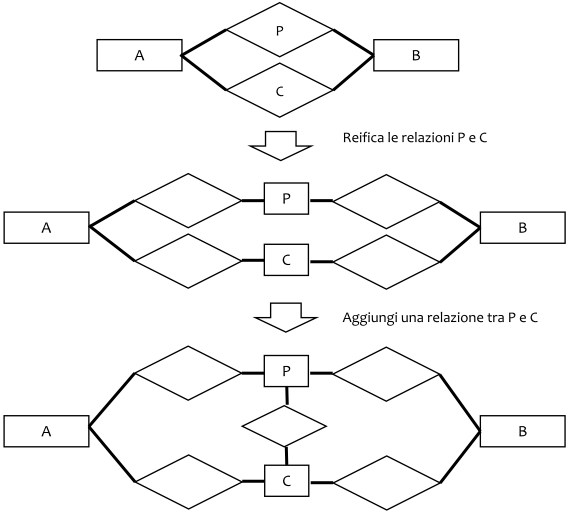
\includegraphics[scale=1]{figures/prevconEXP.png}
\caption{ Divisione della relazione. P e C stanno rispettivamente per Prevenire e Consumare} 
\end{figure}
\end{center}

\begin{flushright}Andrea Camisa\\Gioele Sforza\\6/10/2016\end{flushright}

\section{DATA CENTRIC APPLICATION}

La lezione di oggi ha lo scopo di analizzare il ciclo di creazione e modellazione di applicazioni che si occupano di database. Per l’ingegneria delle applicazioni Data Centric si utilizza un approccio differente: 

\underline{MAPPING ALGORITHM} Trasforma i diagrammi E.R. in tabelle relazionali:

\begin{itemize}

\item{\underline{CONCEPTUAL MODEL}} (ER DIAGRAM);
\item{\underline{LOGICAL MODEL}} – RELATIONAL MODEL (Concetti Astratti);   
\item{\underline{PHYSICAL MODEL}} (REAL DATABASE – MySQL).

\end{itemize}

Un database è un insieme di relazioni $R_i$ e vincoli $C_j$:

\[
	DB = \{R_i,\ C_j\}
\]

Le relazioni sono le tabelle, i vincoli sono le regole che gestiscono le tabelle. Ci sono dei livelli per la costruzione di un database: 

\begin{itemize}

\item{\textbf{PRESENTATION LAYER – P.L.}};
\item{\textbf{BUSINESS RULE LAYER – B.R.L.}};
\item{\textbf{DATABASE LAYER – D.L.}};

\end{itemize}

\subsection{USER TYPES}

Gli User Types sono gli agenti che estraggono le informazioni da Database in modo differente utilizzando il medesimo software. Per ognuno di essi bisogna progettare quindi diverse interfacce e diverse regole di accesso al DB:

\begin{center}
\begin{figure}[H]
\centering
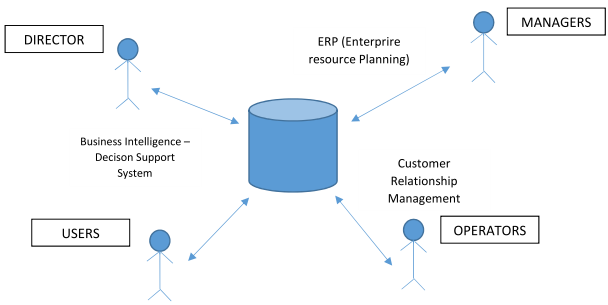
\includegraphics[scale=0.8]{figures/ut.png}
\caption{User Types} 
\end{figure}
\end{center}

\subsection{ESEMPIO}

Usiamo un’applicazione esempio per analizzare lo schema appena spiegato (DL, BRL, PL):

\begin{center}
\begin{figure}[H]
\centering
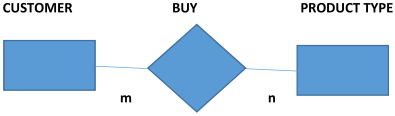
\includegraphics[scale=1]{figures/cbuypt.png}
\caption{Customer Buys Product Type} 
\end{figure}
\end{center}

In questo esempio gli UserTypes sono i Customers e i Sellers e sono per lo più statici, cioè non cambiano. Mentre i Product Type sono più dinamici in quanto rapprensentano le transazioni economiche. 

\begin{center}
\begin{figure}[H]
\centering
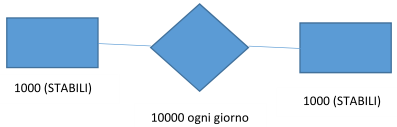
\includegraphics[scale=1]{figures/cbuypt_alim.png}
\caption{Customer Buys Product Type - Dinamicità} 
\end{figure}
\end{center}

$\leftarrow$ La dinamicità della relazione è molto più alta rispetto alle altre due entità. Come facciamo a estrarre differenti info per le diverse tipologie di users? Si userà una forma semplificata del \textbf{Mapping Algorithm}.

\subsection{SIMPLIFIED MAPPING ALGORITHM}

\begin{itemize}

\item \textbf{Ogni Entity Type diventa una tabella e i loro attributi diventano i nomi delle colonne}. Customer, products diventano tabelle, con i relativi attributi. Ogni customer diventerà un record della tabella Customer:

\begin{center}
\begin{figure}[H]
\centering
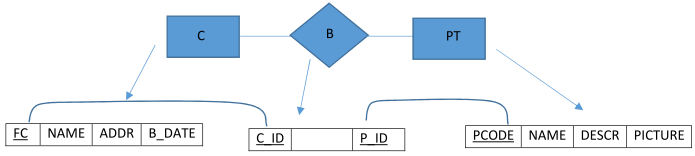
\includegraphics[scale=0.8]{figures/cbuypt_mapping.png}
\caption{Customer Buys Product Type - Mapping} 
\end{figure}
\end{center}

\item \textbf{Ogni Relation Types diventa una tabella}. E’ sempre vero in un solo caso, ovvero quando la relazione è “molti a molti” (n:m):

\begin{itemize}

\item \textbf{Collegare la chiave esterna (F.K.) a ogni entità};
\item \textbf{Completare la tabella con tutti gli attributi presenti della Relation Type}.

\end{itemize}

\begin{itemize}

\item Nel caso \textbf{n:m} si crea quello che si chiama \textbf{Relational Schema of DB};

\item Nel caso della relazione \textbf{1:n}, bisogna includere la tabella della relazione nella tabella finale  dell’entità “\textbf{n}” 

\begin{center}
\begin{figure}[H]
\centering
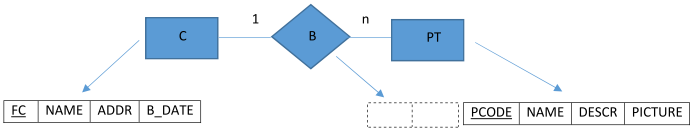
\includegraphics[scale=0.8]{figures/cbuypt1n_mapping.png}
\caption{Customer Buys Product Type - 1:n Mapping} 
\end{figure}
\end{center}

\item Nel caso della relazione \textbf{1:1} si può includere la tabella della relazione in una delle due entità oppure creare una sola tabella:

\begin{center}
\begin{figure}[H]
\centering
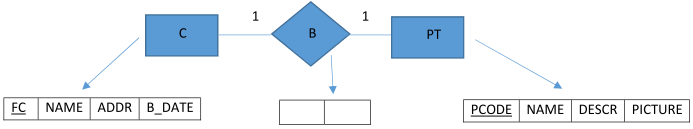
\includegraphics[scale=0.8]{figures/cbuypt11_mapping.png}
\caption{Customer Buys Product Type - 1:1 Mapping} 
\end{figure}
\end{center}

\end{itemize}

\end{itemize}

Se cancello un record da una tabella entità, verrà cancellato ogni record relativo presente nella tabella relazione. Il discorso non vale tra tabelle entità diverse, poiché indipendenti tra loro. Riferendoci all’esempio precedente se ad esempio viene cancellato un customer, ogni transazione riferita a lui viene cancellata, lo stesso vale per i prodotti.  

\subsection{PRESENTATION LAYER FOR CUSTOMER OR DIRECTOR}

Avremo differenti livelli di presentazione, uno per il customer e uno per il direttore del negozio. Per il Customer la Web Application si vedrà come:

\begin{center}
\begin{figure}[H]
\centering
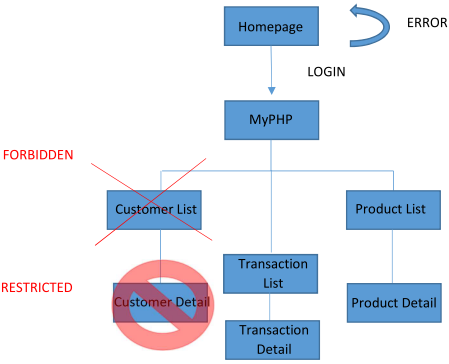
\includegraphics[scale=1]{figures/plcd.png}
\caption{\textbf{Navigation Model of a Website For Customer}}
\end{figure}
\end{center}

Un’altra soluzione potrebbe essere: 

\begin{center}
\begin{figure}[H]
\centering
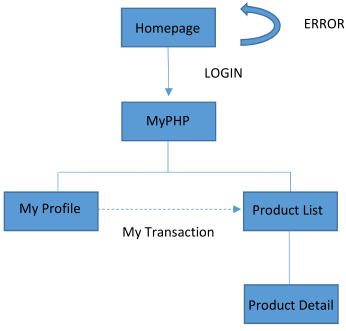
\includegraphics[scale=1]{figures/plcd2.png}
\caption{\textbf{Navigation Model of a Website For Customer} - Another solution}
\end{figure}
\end{center}

Per il Director invece, la Web Application si vedrà come: 

\begin{center}
\begin{figure}[H]
\centering
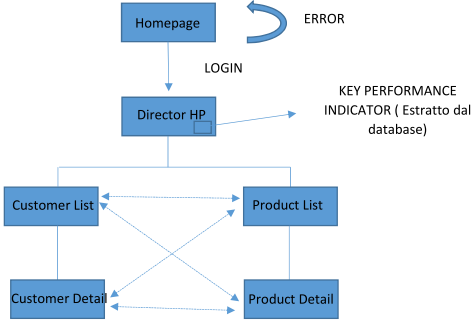
\includegraphics[scale=1]{figures/pld.png}
\caption{\textbf{Navigation Model of a Website For Director}}
\end{figure}
\end{center}

Il direttore ha la possibilità di creare o cancellare i prodotti e di modificare gli attributi di essi. Inoltre può ottenere informazioni sui Customers e quindi potrà poi effettuare delle scelte strategiche per migliorare le vendite con pubblicità o sconti mirati. 

\subsection{BUSINESS RULE LAYER}

Man mano che si sale nella piramide abbiamo bisogno di aggregare le informazioni fino ad avere delle info sempre più riassuntive.

Quando si realizza un progetto c’è bisogno di definire: 

\begin{itemize}

\item CONTEXT \& PROBLEM DEFINITION (2 PAGINE);
\item GOAL \& STAKEHOLDERS;
\item REQUIREMENTS \& CONSTRAINTS;  
\item DATA MODEL:

\begin{itemize}

\item ER DIAGRAM;
\item RELATIONAL MODEL;
\item PHYSICAL MODEL.

\end{itemize}

\item SYSTEM MODELS;
\item SOFTWARE MODELS (MODEL VIEW CONTROLLER):

\begin{itemize}

\item STATE MODEL;
\item PRESENTATION MODEL:

\begin{itemize}

\item IN THE LARGE NAVIGATION (Modello per mostrare le pagine e le connessioni fra di esse);
\item IN THE SMALL NAVIGATION (Modello per analizzare ogni aspetto singolarmente);
\end{itemize}
\end{itemize}
  
\item TEST MODEL;
\item DEPLOYMENT STRATEGY.

\end{itemize}

\section{LIST VIEW and DETAIL VIEW}

Questi due concetti provengono dai sistemi operativi (WINDOWS, MACOS, XWINDOWS/UNIX) e nascono dall’idea comune detta WIMP INTERFACE:

\begin{itemize}

\item WINDOWS = Diversi spazi di lavoro per diverse operazioni (MULTITASKING);
\item ICONS = Oggetti Interattivi;
\item MENUS = Metodi associati ai propri oggetti;
\item POINTERS = Selezionare un oggetto specifico.

\end{itemize}

Da questa metafora nasce l’idea di LIST VIEW e DETAIL VIEW. Se ad esempio apro il Desktop ottengo una lista di oggetti, se invece interagisco con uno di essi ottengo informazioni dettagliate. 

\begin{itemize}

\item{\textbf{LIST VIEW}}

List View può essere una tabella nella quale sono presenti dei metodi well-known come:

\begin{itemize}

\item DELETE OBJECT;
\item SORT;
\item (MOVE);
\item COPY (DUPLICATE OBJECT);
\item INSERT EMPTY OBJECT;
\item FILTER;
\item RENAME;
\item SEARCH (FIND).

\end{itemize}

Altri esempi di List View possono essere una Cartina Geografica, il Desktop o una cartella, un Sets o un Tree. 

\item{\textbf{DETAIL VIEW}}

I metodi well-known della Detail View possono essere:

\begin{itemize}

\item CHANGE (UPDATE);
\item CREATE;
\item DELETE;
\item READ.

\end{itemize}

\end{itemize}

\begin{flushright}Angelo Cotardo\\Francesco Filieri\\12/10/2016\end{flushright}

\begin{center}
\begin{figure}[H]
\centering
\includegraphics[scale=1]{figures/dbut.png}
\caption{Database and User Types}
\end{figure}
\end{center}

Continuiamo con una discussione più dettagliata riguardo i design patterns. Nella scorsa lezione abbiamo esplorato l’intera catena che inizia dal modello e termina con le applicazioni. Il database è un luogo in cui differenti tipi di utente possono svolgere molteplici azioni, ognuno di essi è collegato a qualche processo, descritto tramite un linguaggio grafico chiamato BPML (Business Process Modeling Language) che descrive i processi in un’organizzazione. 
Parleremo di BUSINESS MODEL, molto importante per i nostri scopi, di DATA MODEL, usato per il database e infine di PRESENTATION MODEL e SYSTEM MODEL. 
Quando parliamo di CONCEPTUAL MODEL, ci riferiamo a tutti i modelli che sono molto usati per raccogliere requisiti e informazioni riguardo a ciò che è necessario fare e per trasformare poi questi in software. Approfondiremo gli aspetti di data modeling. 
Abbiamo già introdotto il concetto di ER che andremo ad espandere con i design patterns e con il concetto di EER (ENHANCED ENTITY RELATIONSHIP). Aggiungeremo poi anche qualche concetto riguardo la modellazione di oggetti (ereditarietà ecc.). 

\subsection{DATA PATTERN}

\textbf{Introduciamo il concetto di DATA PATTERN}

Consideriamo il seguente schema:

\begin{center}
\begin{figure}[H]
\centering
\includegraphics[scale=1]{figures/cbuyp.png}
\caption{Customer Buys Product Provided By Provider}
\end{figure}
\end{center}

Stiamo considerando lo scenario in cui un consumatore compra dei prodotti, i quali sono forniti da più fornitori. Osservando gli attributi delle relazioni e delle entità descritte, oltre alla quantità, al tipo di prodotto acquistato e alla data di acquisto, si è definito l’attributo “price” che compare per ben tre volte come attributo delle due relazioni e dell’entità PRODUCT. 

Il significato che assume tale attributo cambia: 

\begin{itemize}

\item{\textit{Selling cost}};
\item{\textit{Catalog cost}};
\item{\textit{Payed cost}}.

\end{itemize}

Nel primo caso esprime il costo del prodotto appena comprato, nel secondo si riferisce al prezzo specificato nel catalogo dei prodotti (non necessariamente selling price deve essere uguale al catalog price ) e nel terzo caso ci si riferisce al prezzo pagato al fornitore riguardo quel prodotto, il quale ovviamente è diverso dal prezzo specificato nel catalogo. 
Il pattern che si è applicato in questo caso (cioè trovare lo stesso attributo in entità o relazioni differenti) prende il nome di PRICE CHAIN (o più in generale ATTRIBUTE CHAIN). 
Un altro tipo di pattern che presentiamo è il PRESENTATION PATTERN che non si focalizza sui dati, bensì sulla loro rappresentazione: l’ARCHIVE PATTERN. È collegato al concetto che quando memorizziamo delle informazioni, esse possono diventare col tempo poco usate.

\begin{center}
\begin{figure}[H]
\centering
\includegraphics[scale=1]{figures/interest_lvl.png}
\caption{Interest Level for Objects}
\end{figure}
\end{center}

Dallo schema si può notare i vari livelli di interesse (LI) per ogni elemento inserito in una list view (cioè le informazioni contenute in tali elementi). In alcuni sistemi quindi, più di un elemento può avere lo stesso livello di interesse, in altri invece, come quelli usati da Google per le ricerche, le informazioni in cima alla lista avranno un livello di interesse elevato rispetto ai successivi elementi. 
Per gestire ciò, viene assegnato ad ogni query un ranking, cioè un indicatore in base al quale ordinare i risultati. Quindi le “risposte” con informazioni più recenti alle “domande” effettuate avranno un ranking più elevato rispetto alle altre. Tali indicatori possono essere assegnati ad esempio sulla base del numero di persone interessate ad un determinato argomento. Un altro esempio del genere, non più basato sul concetto di ranking, può essere quello di una email software, in cui le email più vecchie sono meno importanti delle ultime ricevute, pertanto ci si basa sul tempo.  
Un esempio in cui tutti gli elementi possono avere lo stesso livello di interesse può essere quello dei contatti Whatsapp, in cui ad ognuno di essi viene data la stessa importanza:

\begin{center}
\begin{figure}[H]
\centering
\includegraphics[scale=1]{figures/whatsapp_rd.png}
\caption{Whatsapp: Receiving Date attribute}
\end{figure}
\end{center}

Possiamo aggiungere a tale entity type un \textbf{ranking attribute} (o altri tipi di attributi che collegano il livello di attenzione ai dati). In questo caso consideriamo l’attributo RECEIVING DATE per produrre un archivio gerarchico: 

\begin{center}
\begin{figure}[H]
\centering
\includegraphics[scale=1]{figures/hierarchical_rd.png}
\caption{Whatsapp: Schema gerarchico costruito sulla base dell'attributo Receiving Date}
\end{figure}
\end{center}

Considerando il caso di una email software, si possono organizzare le email ricevute per categorie: anni, mesi, settimane, giorni ecc. Si mette quindi più attenzione alle email ricevute di recente rispetto alle più vecchie (viene assegnato un ranking basato sul tempo). 

\subsubsection{EXAMPLE}

consideriamo il seguente scenario 

\begin{center}
\begin{figure}[H]
\centering
\includegraphics[scale=1]{figures/pppbuy.png}
\caption{Relazione ternaria con PART, PROJECT, PROVIDER}
\end{figure}
\end{center}

Possiamo decidere di usare una relazione ternaria perché tre relazioni binarie non sono sufficienti per dire che una parte specifica è stata fornita da uno specifico fornitore ad uno specifico team (o project).  
Una relazione ternaria quindi collega i tre oggetti nello stesso tempo, cosa che non succederebbe se usassimo tre relazioni binarie. Per dimostrare che la quantità di informazioni è variata possiamo usare il concetto di reificazione. Per trasformare una relazione abbiamo infatti bisogno di un nuovo schema in cui compaiono tre relazioni binarie più una nuova entità (PROVISIONING): 

\begin{center}
\begin{figure}[H]
\centering
\includegraphics[scale=1]{figures/ppp_extended.png}
\caption{Reificazione della Relazione ternaria con PART, PROJECT, PROVIDER}
\end{figure}
\end{center}

Per verificare la cardinalità delle partecipazioni di ogni entità alla relazione ternaria, focalizziamo il nostro punto di vista su ciascuna di esse, vedendo le parti rimanenti del DB come una coppia. 
Ad esempio, concentrandoci sull’entità PART la relazione con la coppia (PROJECT, PROVIDER) è di tipo a molti (n), in quanto ci sono più parti che possono essere fornite da differenti fornitori per differenti progetti. Nello stesso modo, concentrandoci sull’entità PROJECT e osservando la relazione con la coppia (PART, PROVIDER), si nota che in un progetto si possono utilizzare più parti diverse da diversi fornitori, pertanto si assegna una relazione a molti (m). Nel caso del PROVIDER la relazione è di tipo a molti (p), perché si possono vedere una o più coppie del tipo (PART, PROJECT). 
Bisogna tener presente che una volta effettuata la reificazione la cardinalità non varia.                           

Supponiamo di avere due entity type con la seguente cardinalità:  

\begin{center}
\begin{figure}[H]
\centering
\includegraphics[scale=1]{figures/cbuyp2.png}
\caption{Customer Buys Product}
\end{figure}
\end{center}

Trasformando tale schema si ricaveranno tre tabelle, due per le entità e un’altra per la relazione (in quanto si ha una cardinalità n:m). Considerando la seguente variante derivata dalla reificazione:

\begin{center}
\begin{figure}[H]
\centering
\includegraphics[scale=1]{figures/cbuyp_checkout.png}
\caption{Enhanced Customer Buys Product}
\end{figure}
\end{center}

si è trasformato la relazione BUY nell’entità SHOPPING SESSION che può essere effettuata da un cliente e che può includere più prodotti. Dal punto di vista delle informazioni potremmo anche chiamare tale entità con il nome di BILL O TICKET, ma non è propriamente corretto in quanto non è un oggetto esistente, ma solo una collezione di informazioni di altri oggetti. 
Tale entità è il risultato della reificazione e non dall’analisi del problema, per tale motivo questa entità si può considerare come una “entity type di seconda classe” perché non è realmente una classe autonoma dalle altre. Una buona modellazione è considerare tale entity type come una weak entity con un proprio customer. 
Il concetto generale di weak entity type è un po’ differente da quello adottato in questo caso, perché un’entità del genere non può essere identificata in modo univoco dai suoi soli attributi, ma dalla primary key dell’entità collegata ad essa, cioè quella del customer (esempio: due notebook identici sono perfettamente uguali nei loro attributi, ciò che li distingue è il proprietario a cui appartengono). 
In questo caso la SHOPPING SESSION differisce in parte dal concetto di entity type dal momento che possiede anche attributi riguardanti il ticket number e la data del ticket, pertanto ha già delle sue informazioni caratteristiche (la sua primary key che la identifica). 
Infine un CUSTOMER può avere più SHOPPING SESSION, ma ciascuna di esse può avere solo un CUSTOMER e pertanto la relazione a molti (n) dello schema di partenza diventa 1:n. D’altra parte una SHOPPING SESSION può includere più prodotti come anche più prodotti possono essere inclusi in più SHOPPING SESSION facendo diventare la relazione a molti (m) una relazione n:m. Quindi la cardinalità dello schema ER di partenza è legata a quella specificata dopo la reificazione. Gli attributi della relazione di partenza diventeranno gli attributi dell’entità derivata dalla reificazione.  

\subsubsection{EXERCISE: PHR (EHR)}

\begin{center}
\begin{figure}[H]
\centering
\includegraphics[scale=1]{figures/phr.png}
\caption{Personal Health Record (PHR)}
\end{figure}
\end{center}

(proviamo ad usare PRICE CHAIN e ARCHIVE PATTERN) 
Questo problema è chiamato PHR (Personal Health Record) (Cartella Sanitaria Elettronica): il paziente si reca dal medico di famiglia, viene informato circa la sua situazione clinica e gli vengono prescritti alcuni test da fare. Il paziente si reca al centro dei test clinici (CTL), oppure in ospedale (H, PH) per radiografie o per altri test. Successivamente i risultati verranno consegnati al medico di famiglia. Questo è uno scenario classico.  
Perché non creare un database online di pazienti, così da mettere tutti i loro report e accedere alle informazioni usando solo username e password? Il problema è abbastanza semplice da descrivere, ma è abbastanza complesso da risolvere. Google creò alcuni anni fa Google Health e Microsoft presentò Microsoft Healthvault, due applicazioni che permettevano di inserire tutte le nostre informazioni nel database. Google e Microsoft hanno realizzato questi database e hanno fallito. Adesso non ci sono soluzioni disponibili in questo ambito.   

Possibili problemi in cui si può incorrere sono:

\begin{itemize}

\item persone anziane;
\item no standard;
\item benefits misunderstanding (i pazienti non comprendono i benefici);
\item i dottori non vogliono l’automazione (power knowledge);
\item aspetti legati alla privacy.

\end{itemize}

Il fallimento di tali sistemi sta anche nel fatto che potremmo essere “bombardati” da tanti annunci riguardanti alcuni specifici rimedi. Se qualcuno pagasse, potrebbe forzare Google a dare informazioni false riguardo la nostra salute. Inoltre le preoccupazioni relative alla privacy sono estremamente importanti e l’interesse economico del mondo dei dati personali della salute è di decine di miliardi di euro. 

\textbf{Analizziamo i requisiti del database di una clinica}.

Quando il paziente arriva in clinica, la receptionist lo ammette e informa il dottore che è arrivato un paziente (è una ammissione tecnica, gli permette l’ingresso). Il dottore a sua volta ammette il paziente che sta aspettando, questa è un’ammissione clinica, perché dal punto di vista medico un dottore dice al paziente che può iniziare una cura/terapia. Il paziente quindi descrive il problema e il dottore fa l’anamnesi (scrive le note e mette tutte le informazioni nella cartella del paziente, nel sistema). I dottori sottoscrivono la prescrizione, i test e invitano i pazienti a sottoporsi ad essi (anche nella stessa clinica). Successivamente delle infermiere effettuano i test e i risultati sono poi inseriti nel sistema. I pazienti potranno visualizzare i risultati dei test a casa sul loro computer.  
Elenchiamo i tipi di utente presenti nello scenario descritto:

\begin{itemize}

\item DOCTOR;
\item RECEPTIONISTS;
\item PATIENTS;
\item NURSES.

\end{itemize}

Descriviamo lo scenario mediante questo semplice schema: 

\begin{center}
\begin{figure}[H]
\centering
\includegraphics[scale=1]{figures/clinics_req.png}
\caption{Clinics - Requirements}
\end{figure}
\end{center}

Possiamo vedere quanto facile e immediato è descrivere un problema in termini di dati scambiati tra i tipi di utente. Il framework che abbiamo visto è molto efficace perché iniziamo a vedere ciò che ci circonda in modo differente. Ci sono: tipi di utente, azioni, informazioni (che sono scambiate tra i vari utenti), tipi di relazioni tra entità. Abbiamo così una buona e immediata descrizione di un problema reale. 

Iniziamo una prima fase di modellazione considerando tre relazioni binarie tra le seguenti entità: 

\begin{center}
\begin{figure}[H]
\centering
\includegraphics[scale=1]{figures/clinics_ER.png}
\caption{Clinics - ER Draft}
\end{figure}
\end{center}


\begin{flushright}Andrea Cuna\\Giuseppe Levantaci\\13/10/2016\end{flushright}

Riprendiamo la modellazione del problema della clinica. Sono sicuramente necessarie le seguenti entity type:

\begin{itemize}

\item PATIENT;
\item DOCTOR;
\item RECEPTIONIST. 

\end{itemize}

Dobbiamo tener conto del fatto che un paziente prenota in anticipo una visita. Quando egli si presenta in ambulatorio, dovrà essere “ammesso” alla visita dal receptionist, il quale ovviamente “informerà” il medico: 

\begin{center}
\begin{figure}[H]
\centering
\includegraphics[scale=1]{figures/clinics_incER.png}
\caption{Clinics - Incremental ER}
\end{figure}
\end{center}

Vediamo ora come specificare l’intervista del dottore al paziente:

\begin{center}
\begin{figure}[H]
\centering
\includegraphics[scale=0.8]{figures/pid.png}
\caption{Doctor Interviews Patient}
\end{figure}
\end{center}

Va ricordato, ora, che le interviste riguardano la storia clinica del paziente, lo stile di vita e il problema medico attuale, e l’assunzione o meno di farmaci, per cui avremo le seguenti relazioni:

\begin{itemize}

\item Il paziente è connesso ad altri pazienti da una relazione (ricorsiva) di parentela (informazione utile per considerare l'eventuale ereditarietà delle malattie): 

\begin{center}
\begin{figure}[H]
\centering
\includegraphics[scale=1]{figures/pirof.png}
\caption{Patient Is Relative Of Patient}
\end{figure}
\end{center}

\item Il paziente è malato:

\begin{center}
\begin{figure}[H]
\centering
\includegraphics[scale=1]{figures/patient_has_disease.png}
\caption{Patient Has Disease}
\end{figure}
\end{center}

\item Il paziente assume medicinali:

\begin{center}
\begin{figure}[H]
\centering
\includegraphics[scale=1]{figures/patient_assume_drug.png}
\caption{Patient Assume Drug}
\end{figure}
\end{center}

\item Ora inseriamo il concetto di stile di vita del paziente (ad esempio se è un fumatore) modellando una nuova entity type: 

\begin{center}
\begin{figure}[H]
\centering
\includegraphics[scale=1]{figures/patient_has_lb.png}
\caption{Patient Has Lifestyle Behavior}
\end{figure}
\end{center}

\end{itemize}

Come si può vedere, queste ultime quattro relazioni tengono traccia delle informazioni che scaturiscono dall’intervista.	

Vediamo ora come si può modellare la prescrizione di medicine, esami, test e indagini cliniche al paziente da parte del dottore:

\begin{itemize}

\item Si potrebbe modellare in questo modo:

\begin{center}
\begin{figure}[H]
\centering
\includegraphics[scale=1]{figures/doctor_prescribe_drug.png}
\caption{Patient Has Lifestyle Behavior}
\end{figure}
\end{center}

\item Potremmo considerare anche: 

\begin{center}
\begin{figure}[H]
\centering
\includegraphics[scale=1]{figures/patient_rpa_drug.png}
\caption{Patient Receives Prescription About Drug}
\end{figure}
\end{center}

\end{itemize}

Ora sappiamo che durante la visita il dottore prescrive le medicine al paziente, inoltre l’intervista è qualcosa che avviene durante la visita. Per questo è possibile applicare la reificazione a VISIT e assumere che durante la visita il paziente dichiari di usare medicine e di avere un certo stile di vita; in questo modo non sarà più necessario specificare la data dell’intervista come attributi delle due relazioni HAS, e si terrà anche conto del dottore.   

\begin{center}
\begin{figure}[H]
\centering
\includegraphics[scale=0.8]{figures/clinics_incER2.png}
\caption{Clinics - Incremental ER 2}
\end{figure}
\end{center}

In precedenza abbiamo detto che durante l'intervista (e quindi durante la visita), il paziente comunica al dottore le medicine che assume, il dottore prescrive al paziente delle medicine e gli diagnostica una malattia. Queste considerazioni ci permettono di associare DISEASE e DRUG a VISIT, invece che a PATIENT.	

In questo modo le relazioni precedenti diventano: 

\begin{center}
\begin{figure}[H]
\centering
\includegraphics[scale=0.8]{figures/clinics_incER3.png}
\caption{Clinics - Incremental ER 3}
\end{figure}
\end{center}

In seguito ad una visita, il medico potrebbe anche prescrivere al paziente un “esame”, il quale verrà effettuato da un “infermiere”, quindi possiamo modellare in questo modo:   

\begin{center}
\begin{figure}[H]
\centering
\includegraphics[scale=1]{figures/clinics_incER4.png}
\caption{Clinics - Incremental ER 4}
\end{figure}
\end{center}

In particolare, NURSE effettua un TEST (nel senso di un esame specifico di un determinato paziente) di tipo TYPE OF TEST (inteso come esame in senso generico, ad esempio “analisi del sangue”), il quale è prescritto da un medico (stiamo utilizzando il pattern Object-Type of object). 
Abbiamo bisogno dunque delle seguenti relation types:

\begin{itemize}

\item DOES (NURSE-DOES-TEST);
\item INSTANCE OF (TEST-INSTANCE OF-TYPE OF TEST);
\item PRESCRIBES (VISIT-PRESCRIBES-TYPE OF TEST).

\end{itemize}
	
La prescrizione del test si può modellare, dunque, in questo modo:

\begin{center}
\begin{figure}[H]
\centering
\includegraphics[scale=0.8]{figures/clinics_incER5.png}
\caption{Clinics - Incremental ER 5}
\end{figure}
\end{center}

\newpage
Il modello ER finale per il nostro problema è il seguente: 

\begin{center}
\begin{figure}[H]
\centering
\includegraphics[scale=0.8]{figures/clinics_finalER.png}
\caption{Clinics - Final ER}
\end{figure}
\end{center}


\section{DBMS}

\subsection{Descrizione dei principali DBMS}

\begin{center}
\begin{figure}[H]
\centering
\includegraphics[scale=0.8]{figures/DBMS.png}
\caption{DBMS}
\end{figure}
\end{center}

Tra i DBMS più conosciuti troviamo:  

\begin{itemize}

\item MySQL;
\item MongoDB;
\item SQLite;
\item PostgreSQL;
\item Oracle;
\item Microsoft SQL Server;
\item Microsoft Access (e il suo competitor OpenOffice Base);
\item Couchbase.

\end{itemize}

Analizziamone alcuni più in dettaglio. 

\begin{itemize}

\item{\textbf{Oracle, Microsoft SQL Server} e \textbf{MySQL}} sono RDBMS, ovvero DBMS “\textbf{relazionali}” (che coprono circa il 90 \% del mercato dei DBMS). Oracle ha un prezzo di circa 60.000 €, SQL Server 10.000 €, mentre MySQL è gratuito, pur essendo in qualche modo paragonabile agli altri due. Oracle e SQL Server sono di fascia “enterprise”, impiegati quindi nell’ambito di grandi aziende (es. banche), mentre MySQL è perfetto per gli studenti universitari che si affacciano al mondo dei database;

\item{\textbf{MongoDB} e \textbf{Couchbase}} sono DBMS “NoSQL”, ovvero NON relazionali, idonei per particolari applicazioni;

\item{\textbf{PostgreSQL}} è un Object Relational DBMS, ovvero presenta alcune caratteristiche tipiche della programmazione orientata agli oggetti. Questo consente un Object-Relational Mapping più preciso;

\item Infine, \textbf{Microsoft Access} e il suo diretto competitor open source \textbf{OpenOffice Base} sono semplici DBMS utilizzati principalmente per la costruzione veloce di prototipi di database.

\end{itemize}


\subsection{Installazione e configurazione di MySQL} 

\begin{itemize}

\item{\textit{Installazione su Microsoft Windows}}

Recarsi al seguente indirizzo: \url{http://dev.mysql.com/downloads/mysql/}; Selezionare il proprio Sistema Operativo ed eseguire il Download.

\begin{center}
\begin{figure}[H]
\centering
\includegraphics[scale=0.8]{figures/mySQLinstaller.png}
\caption{MySQL Installer Download}
\end{figure}
\end{center}

Prima di effettuare l’installazione eseguire il seguente download:

\begin{center}
\begin{figure}[H]
\centering
\includegraphics[scale=0.8]{figures/visualc++.png}
\caption{Visual C++ Redistributable Packages download}
\end{figure}
\end{center}

Dopo il download selezionare ed avviare l’installazione, il file avrà nome: \newline “ mysql-installercommunity-x.x.x.x-dmr.msi “ dove x.x.x.x sarà il numero di versione, verrà poi visualizzata la seguente schermata:

\begin{center}
\begin{figure}[H]
\centering
\includegraphics[scale=1]{figures/mySQLinstaller_splash.png}
\caption{MySQL Installer Splash-Screen}
\end{figure}
\end{center}

Verrà visualizzata la seguente schermata: 

\begin{center}
\begin{figure}[H]
\centering
\includegraphics[scale=0.8]{figures/mySQLinstaller_wizard.png}
\caption{MySQL Installer Wizard}
\end{figure}
\end{center}

Accettare i termini di licenza e poi proseguire nell’installazione. 

Nella schermata successiva selezionare quanto evidenziato: 

\begin{center}
\begin{figure}[H]
\centering
\includegraphics[scale=1]{figures/mySQLinstaller_wizard2.png}
\caption{MySQL Installer Wizard 2}
\end{figure}
\end{center}

E nella schermata successiva configurare i pacchetti come riportati in figura: 

\begin{center}
\begin{figure}[H]
\centering
\includegraphics[scale=1]{figures/mySQLinstaller_wizard3.png}
\caption{MySQL Installer Wizard 3}
\end{figure}
\end{center}

e quindi proseguire nell’installazione cliccando due volte sul tasto “ Next $>$ “. Si raggiungerà la seguente schermata:

\begin{center}
\begin{figure}[H]
\centering
\includegraphics[scale=0.8]{figures/mySQLinstaller_wizard4.png}
\caption{MySQL Installer Wizard 4}
\end{figure}
\end{center}

Al termine dell’installazione verrà installato, oltre al server, il software “MySQL WorkBench” il quale è utile per creare e gestire le tabelle dei database contenuti nel server. Al primo avvio del server verrà richiesto di inserire una password di amministratore: qui si può inserire una password a scelta che dovrà essere ricordata per eseguire l’accesso negli usi successivi. 

\item{\textit{INSTALLAZIONE SU MACOS}}

Recarsi allo stesso URL indicato in precedenza, selezionare il sistema operativo MacOS ed eseguire il download del pack dmg. In seguito, una volta aperto il pack dmg ed avviata l’installazione del pack pkg al suo interno, si otterrà questa schermata:

\begin{center}
\begin{figure}[H]
\centering
\includegraphics[scale=1]{figures/mySQLinstaller_macOS_wizard.png}
\caption{MySQL Installer MacOS Wizard}
\end{figure}
\end{center}

cliccando su continua si dovrà poi accettare la licenza:

\begin{center}
\begin{figure}[H]
\centering
\includegraphics[scale=1]{figures/mySQLinstaller_macOS_wizard2.png}
\caption{MySQL Installer MacOS Wizard 2}
\end{figure}
\end{center}

Successivamente nella schermata successiva basterà cliccare su “Installa” e verrà avviata l’installazione durante la quale sarà richiesta la password di amministratore: 

\begin{center}
\begin{figure}[H]
\centering
\includegraphics[scale=1]{figures/mySQLinstaller_macOS_wizard3.png}
\caption{MySQL Installer MacOS Wizard 3}
\end{figure}
\end{center}

Alla fine dell’installazione verrà visualizzata una finestrella contenente la password di amministratore generata automaticamente: 

\begin{center}
\begin{figure}[H]
\centering
\includegraphics[scale=1]{figures/mySQLinstaller_macOS_wizard4.png}
\caption{MySQL Installer MacOS Wizard 4}
\end{figure}
\end{center}

Dopo di che sarà possibile avviare il Server tramite le impostazioni:

\newpage

\begin{center}
\begin{figure}[H]
\centering
\includegraphics[scale=1]{figures/macOS_mySQL_settings.png}
\caption{Mac OS Settings MySQL}
\end{figure}
\end{center}

\begin{center}
\begin{figure}[H]
\centering
\includegraphics[scale=1]{figures/mySQL_serverstatus.png}
\caption{MySQL Server Status}
\end{figure}
\end{center}
\newpage

Ora bisogna installare “MySQL WorkBench”: Eseguire il download da questo link: \url{http://dev.mysql.com/downloads/workbench/}. Seguendo i passaggi riportati sopra per la selezione del sistema operativo. Una volta eseguito il download aprire il pack dmg ottenendo: 

\begin{center}
\begin{figure}[H]
\centering
\includegraphics[scale=1]{figures/mySQL_workbench_splash.png}
\caption{MySQL Workbench Splash-Screen}
\end{figure}
\end{center}

E come suggerisce l’immagine, spostare l’applicazione nella cartella per eseguire l’installazione.

\end{itemize}

\subsection{PRIMO CONTATTO CON MYSQL WORKBENCH}

Aprire il programma. Si troverà la seguente schermata:

\begin{center}
\begin{figure}[H]
\centering
\includegraphics[scale=0.8]{figures/mySQL_workbench_home.png}
\caption{MySQL Workbench Home Screen}
\end{figure}
\end{center}

Cliccando sul “+” accanto a MySQL Connections si potrà aggiungere una nuova connessione ad un database SQL già avviato ( vedi passaggi precedenti ) visualizzando una schermata che chiederà di inserire la password da amministratore:  

\begin{center}
\begin{figure}[H]
\centering
\includegraphics[scale=1]{figures/mySQL_login.png}
\caption{MySQL Login Screen}
\end{figure}
\end{center}

Una volta eseguito l’accesso, si avrà la seguente schermata: 

\begin{center}
\begin{figure}[H]
\centering
\includegraphics[scale=0.8]{figures/mySQL_workbench_initial.png}
\caption{MySQL Workbench Initial Screen}
\end{figure}
\end{center}

Tramite il tasto “ Server Status“ è possibile visionare lo stato del server e “Avviare/Fermare” l’istanza del server SQL:

\begin{center}
\begin{figure}[H]
\centering
\includegraphics[scale=0.8]{figures/mySQL_workbench_serverstatus.png}
\caption{MySQL Workbench Server Status}
\end{figure}
\end{center}

Tramite il tasto “+” posizionato a destra della scritta Models in basso a sinistra:  
si potrà creare un nuovo modello, visualizzando la seguente schermata:  

\begin{center}
\begin{figure}[H]
\centering
\includegraphics[scale=0.8]{figures/mySQL_workbench_model.png}
\caption{MySQL Workbench - Model}
\end{figure}
\end{center}

Cliccando su “Add Table” ( evidenziato nella figura precedente ) si potrà inserire una nuova tabella nel nostro modello e la schermata diventerà: 

\begin{center}
\begin{figure}[H]
\centering
\includegraphics[scale=0.8]{figures/mySQL_workbench_addtable.png}
\caption{MySQL Workbench - Add Table}
\end{figure}
\end{center}

In basso al centro verrà visualizzata la struttura della nuova tabella. Tramite “Name” sarà possibile rinominarla. Costruire una tabella come quella riportata in figura:  

\begin{center}
\begin{figure}[H]
\centering
\includegraphics[scale=0.8]{figures/mySQL_workbench_newtable.png}
\caption{MySQL Workbench - New Table}
\end{figure}
\end{center}

in cui:

\begin{itemize}

\item{\textbf{id}} è la CHIAVE PRIMARIA (PK) NON NULLA (NN) e AUTO INCREMENTANTE (AI) identificata come un intero;
\item{\textbf{first\_name} e \textbf{last\_name}} sono Nome e Cognome della persona identificati come un insieme di stringhe di massimo 45 caratteri;
\item{\textbf{birth\_date}} è la data di nascita della persona ed è identificato come un oggetto DATE (ossia una data in formato internazionale AAAA-MM-GG);
\item{\textbf{picture}} è invece l’immagine di una persona identificata nel database con un oggetto BLOB ossia un Binary Long OBject;

\end{itemize}

Ora in alto nei menù si dovrà selezionare : “ Database $\rightarrow$ Forward Engineering ” per eseguire il salvataggio del nostro modello sul server a cui siamo collegati, tramite questo semplice wizard: 

\begin{center}
\begin{figure}[H]
\centering
\includegraphics[scale=1]{figures/mySQL_workbench_FE.png}
\caption{MySQL Workbench - Forward Engineering}
\end{figure}
\end{center}

qui va selezionato il server di destinazione, in seguito selezionare le opzioni necessarie (per ora lasciamo tutto invariato) 

\begin{center}
\begin{figure}[H]
\centering
\includegraphics[scale=0.8]{figures/mySQL_workbench_FE2.png}
\caption{MySQL Workbench - Forward Engineering step 2}
\end{figure}
\end{center}

Poi bisognerà selezionare gli oggetti che si vogliono ottenere da questa esportazione:

\begin{center}
\begin{figure}[H]
\centering
\includegraphics[scale=1]{figures/mySQL_workbench_FE3.png}
\caption{MySQL Workbench - Forward Engineering step 3}
\end{figure}
\end{center}

Verrà mostrato il codice SQL di creazione del modello prima di essere esportato sul server: 

\begin{center}
\begin{figure}[H]
\centering
\includegraphics[scale=0.8]{figures/mySQL_workbench_FE4.png}
\caption{MySQL Workbench - Forward Engineering step 4}
\end{figure}
\end{center}

Infine si esegue il salvataggio:

\begin{center}
\begin{figure}[H]
\centering
\includegraphics[scale=1]{figures/mySQL_workbench_FEfinal.png}
\caption{MySQL Workbench - Forward Engineering - Save}
\end{figure}
\end{center}

Andando ora a rivedere il contenuto del server (sempre tramite il Workbench) troveremo un nuovo database chiamato \textbf{mydb}:

\begin{center}
\begin{figure}[H]
\centering
\includegraphics[scale=0.8]{figures/mySQL_workbench_mydb.png}
\caption{MySQL Workbench - mydb RECAP}
\end{figure}
\end{center}

cliccando col tasto destro sulla tabella \textbf{person} e selezionando: “ Select Row – Limit 1000 ” verrà visualizzato il contenuto della tabella caricata sul server con la seguente schermata: 

\begin{center}
\begin{figure}[H]
\centering
\includegraphics[scale=0.8]{figures/mySQL_workbench_person.png}
\caption{MySQL Workbench - person set on server}
\end{figure}
\end{center}

dove nella parte in alto viene visualizzata la “QUERY”, e in basso il risultato (ovviamente ora viene visualizzata una tabella vuota). A questo punto fare doppio click nella selezione rossa nell’immagine, in corrispondenza di first\_name, e inserire il nome. Continuare così per il resto dei campi e poi premere invio, in questo modo si inseriranno i dati all’interno della tabella. Bisognerà ottenere un risultato come il seguente: 

\begin{center}
\begin{figure}[H]
\centering
\includegraphics[scale=1]{figures/mySQL_workbench_personinsert.png}
\caption{MySQL Workbench - Insert new people}
\end{figure}
\end{center}

In seguito in basso a sinistra si troverà il tasto “Apply”:

\begin{center}
\begin{figure}[H]
\centering
\includegraphics[scale=0.8]{figures/mySQL_workbench_apply.png}
\caption{MySQL Workbench - Apply}
\end{figure}
\end{center}

Si aprirà il seguente wizard in cui sarà visualizzata la QUERY da eseguire sul database:

\begin{center}
\begin{figure}[H]
\centering
\includegraphics[scale=0.8]{figures/mySQL_workbench_prequerywizard.png}
\caption{MySQL Workbench - Pre-query wizard}
\end{figure}
\end{center}

Cliccando su “Apply” verrà eseguita la query ottenendo il seguente risultato: 

\begin{center}
\begin{figure}[H]
\centering
\includegraphics[scale=1]{figures/mySQL_workbench_postscriptwizard.png}
\caption{MySQL Workbench - Post-query wizard}
\end{figure}
\end{center}

Provare ora ad eseguire le QUERY:

\begin{itemize}

\item{}

\begin{lstlisting}[language=SQL]
SELECT * FROM mydb.person WHERE first_name = 'Mario'
\end{lstlisting}

\item{}

\begin{lstlisting}[language=SQL]
SELECT * FROM mydb.person WHERE first_name = 'M'
\end{lstlisting}

\item{}

\begin{lstlisting}[language=SQL]
SELECT * FROM mydb.person WHERE first_name = 'mario'
\end{lstlisting}

\end{itemize}

e proseguire facendo varie prove, modificando le QUERY. 

\begin{flushright}Marco D'Amato\\Marco Mameli\\13/10/2016\end{flushright}


\section{IMPORTANZA MODELLI}

\subsection{IMPORTANZA MODELLO DATI}

Tra i vari modelli dell’ingegneria del software, il modello dati ha una rilevanza particolare in quanto influisce in maniera determinante sulle funzionalità dell’applicazione. Tuttavia, i vari schemi di un sistema software sono:

\begin{itemize}

\item{DATABASE MODEL}: come già accennato, il più importante;
\item{BUSINESS MODEL}: vagamente simile al diagramma dei casi d’uso, ha il compito di esplicare le ragioni presenti dietro lo sviluppo di un sistema software. Consiste nella creazione di scenari, nei quali i prodotti applicativi servono a creare delle soluzioni a problemi specifici. Questi schemi mostrano lo scambio di valore intorno all’applicazione (E3 VALUE);
\item{MODELLO DI SISTEMA}: importante per la scalabilità e la realizzabilità dell’applicazione;

\item{PRESENTATION MODEL}: in questo caso si parla di visibility design, dove i vari attori sono inseriti in un diagramma in cui sono riportate le varie funzioni relative ad ognuno di essi.

\begin{center}
\begin{figure}[H]
\centering
\includegraphics[scale=1]{figures/cbuyp3.png}
\caption{Customer Buys Product}
\end{figure}
\end{center}

Ultimamente quello dei disappearing computer è uno dei più interessanti ambiti di ricerca, dove per computer si intendono smart devices e smart processes: l’obiettivo è quello di rendere smart la parte relativa all’inserimento e al rilevamento dati;

\item{TEST}: relativamente meno importante degli altri, ma validi da un punto di vista economico in quanto spesso è il collaudo a sbloccare i finanziamenti per il software. 
 
\end{itemize}

\subsection{IMPORTANZA INFORMAZIONE}

\begin{center}
\begin{figure}[H]
\centering
\includegraphics[scale=1]{figures/dmo.png}
\caption{Anthony's DMO Pyramid}
\end{figure}
\end{center}

Nella progettazione di un sistema software è importante progettare interfacce diverse per tipo di utente, creando diagrammi di comunicazione on the large per ogni utente. 

\begin{center}
\begin{figure}[H]
\centering
\includegraphics[scale=1]{figures/otl.png}
\caption{On the Large Communication Diagram}
\end{figure}
\end{center}

Esempio sui canali di comunicazione:

\begin{itemize}

\item Lettori leggono prodotto Autori;
\item Autori leggono feedback dei Lettori;
\item Lettori leggono feedback degli altri Lettori (casi generici Booking.com, TripAdvisor);
\item Community di Autori. 

\end{itemize}

\section{DIAGRAMMI EER}

Le tre caratteristiche della progettazione ad oggetti sono: Ereditarietà, Polimorfismo, Incapsulamento. Quest’ultimo non è presente nei Database, in quanto le entità non sono trasparenti; il polimorfismo è una componente essenziale per la programmazione, mentre non lo è per i dati. Per aggiungere l’Ereditarietà ai diagrammi E-R (Entity-Relationship) sono stati introdotti i diagrammi EER (Enhanced Entity Relationship).

\begin{center}
\begin{figure}[H]
\centering
\includegraphics[scale=1]{figures/EER.png}
\caption{Diagramma EER}
\end{figure}
\end{center}

La modifica apportata allo schema di riferimento Cliente - Acquista - Prodotto rappresenta la specializzazione dell’entità cliente (si noti il simbolo di inclusione insiemistica). A questo punto si presentano due possibili situazioni:

\begin{itemize}

\item

\begin{center}
\begin{figure}[H]
\centering
\includegraphics[scale=1]{figures/EERset1.png}
\caption{Diagramma di Eulero-Venn per EER disjoint entities}
\end{figure}
\end{center}

Le due entità pur essendo incluse nell’entità parent, non hanno elementi in comune. In questo caso si dicono disgiunte, e nel cerchio presente nel simbolo di specializzazione del diagramma EER si inserisce la lettera “d” (disjoint):

\begin{center}
\begin{figure}[H]
\centering
\includegraphics[scale=1]{figures/disjoint.png}
\caption{Disjoint Inheritance for EER}
\end{figure}
\end{center}

\item

\begin{center}
\begin{figure}[H]
\centering
\includegraphics[scale=1]{figures/EERset2.png}
\caption{Diagramma di Eulero-Venn per EER overlapping entities}
\end{figure}
\end{center}

Le due entità potrebbero avere elementi in comune, come nel caso sotto riportato. In tal caso si inserisce la lettera “o” (overlap):

\begin{center}
\begin{figure}[H]
\centering
\includegraphics[scale=1]{figures/overlapping.png}
\caption{Overlapping Inheritance for EER}
\end{figure}
\end{center}

\end{itemize}

Esiste un importante differenza tra specializzazione e generalizzazione: La prima, effettuata a priori è sempre possibile, mentre la seconda non sempre. Nell’ultimo caso si può scoprire a posteriori che oggetti diversi appartengono alla stessa classe rendendo difficile per il software aggiornare la struttura dati. Un modo fattibile di implementare la generalizzazione è attraverso la UNION. Tale elemento di modellazione concettuale è rappresentato come sotto, dove in tal caso si inserisce il simbolo di “u” (union):

\begin{center}
\begin{figure}[H]
\centering
\includegraphics[scale=0.8]{figures/union.png}
\caption{Union for EER}
\end{figure}
\end{center}

A differenza dell’Overlap, in questo caso le entità child mantengono i loro attributi ma sono unite sotto l’entità parent risolvendo parzialmente il problema: infatti nel caso della union si ha che fare con insiemi di oggetti diversi aventi attributi diversi. Si noti che l’entità Vehicle non contiene niente tranne che l’ID che però non è presente a livello concettuale ma solo a livello logico (dove sono presenti le tabelle). 

\subsection{SCHEMA EER CAPITOLO 4} 

\begin{center}
\begin{figure}[H]
\centering
\includegraphics[scale=0.7]{figures/EERschema_cpt4.png}
\caption{\textbf{SCHEMA EER CAPITOLO 4}}
\end{figure}
\end{center}

Nel diagramma sopra riportato la doppia linea rappresenta una specializzazione esclusiva, a indicare una partecipazione totale.  Le due diverse specializzazioni disgiunte sono entrambe ortogonali, in quanto le entità child sono indipendenti l’una dall’altra. Nel caso di ereditarietà multipla non sempre le speciali portano ad alberi aperti: come si evince dal precedente diagramma possono esserci maglie chiuse. Il caso peggiore di queste situazioni si presenta quando gli attributi vengono gestiti due volte, anche se si tratta di un evento abbastanza raro.


\subsection{ESERCIZIO SVOLTO IN CLASSE}

\begin{center}
\begin{figure}[H]
\centering
\includegraphics[scale=0.7]{figures/museum.png}
\caption{\textbf{Museum Exercise ER}}
\end{figure}
\end{center}


\begin{flushright}Ippazio Alessio\\Simone Dongiovanni\\19/10/2016\end{flushright}